\documentclass[usenatbib]{tjaa}

\usepackage[utf8]{inputenc}
\usepackage{lipsum}
\usepackage{cite}
\usepackage{amsmath,amssymb,amsfonts}
\usepackage{algorithmic}
\usepackage{graphicx}
\usepackage{textcomp}
\usepackage{xcolor}
\usepackage{wrapfig}
\usepackage{subcaption}
\usepackage{subfig}
\usepackage{pdfpages}
\usepackage{tcolorbox}
\usepackage{float}
\usepackage{placeins}

\usepackage[font=small,labelfont=bf]{caption} % If you are using the caption package
\usepackage{fancyhdr}  % To customize headers and footers
\usepackage{graphicx}  % For including images
\usepackage{lipsum}    % For dummy text (optional)

\pagestyle{fancy}
% \fancyhf{}  % Clear default header and footer
% \fancyhead[L]{2024 27th International Conference on Computer and Information Technology (ICCIT)
% 20-22 December 2024, Cox’s Bazar, Bangladesh}  % Left side header
\fancyhead[R]{Page \thepage}  % Right side header with page number

\newsavebox\verbbox

\vspace{-10cm}
\title[]{\centering Machine Learning and IoT Based Traffic Management System: Prioritizing Emergency Vehicles and Reducing Congestion}


% \author[]{%
% First Author\autid{1}{0000-0000-0000-0000}\,
% A. N. Other\autid{2}{0000-0000-0000-0000},
% Third Author\autid{2,3}{0000-0000-0000-0000}
% \newauthor
% \\
% \adrid{1}University, Department, City Post Code, Country\\
% \adrid{2}Department, Institution, Street Address, City Postal Code, Country\\
% \adrid{3}Another Department, Different Institution, Street Address, City Postal Code, Country%
% }



\author[]{
    \begin{minipage}[t]{0.32\textwidth}
        \centering
        \normalsize
         Saied Afnan
        % \autid{1}{0000-0000-0000-0000}\
        \\ 
        \textit{\normalsize Computer Science and Engineering} \\
        \normalsize Shahjalal University of Science and Technology \\
        \normalsize Sylhet, Bangladesh \\
        \normalsize afnan.cse19.sust@gmail.com
    \end{minipage}
    \hspace{0.01\textwidth} % Adds a little more gap between columns
    \begin{minipage}[t]{0.32\textwidth}
        \centering
        \normalsize
        Alomgir Hossain
        % \autid{2}{0000-0000-0000-0000}\
        \\
        \textit{\normalsize Computer Science and Engineering} \\
        \normalsize Shahjalal University of Science and Technology \\
        \normalsize Sylhet, Bangladesh \\
        \normalsize a.h.joy066@gmail.com
    \end{minipage}
    \hspace{0.01\textwidth} % Adds a little more gap between columns
    \begin{minipage}[t]{0.32\textwidth}
        \centering
        \normalsize
        M. Shahidur Rahman
        % \autid{3}{0000-0000-0000-0000}\
        \\
        \textit{\normalsize Computer Science and Engineering} \\
        \normalsize Shahjalal University of Science and Technology \\
        \normalsize Sylhet, Bangladesh \\
        \normalsize rahmanms@sust.edu
    \end{minipage}
}

\begin{document}
\label{firstpage}
\pagerange{\pageref{firstpage}--\pageref{lastpage}}
\maketitle{M00-000}

\begin{abstract}
Traffic crowds and futility present vital challenges for urban areas in developing nations, specifically in Dhaka, Bangladesh. The rapid fixity of urbanization, limited road infrastructure, and the high appearance of mixed traffic—consisting of rickshaws, motorcycles, buses, cars, and other vehicles—contribute to intense rush and delays. This technology proposes an IoT-enabled traffic regulation system that integrates the YOLOv10 (You Only Look Once) Machine Learning Model for real-time traffic regulation. to detect and classify vehicles, pedestrians, and emergency vehicles, facilitating intelligent traffic signal adjustments based on traffic density The process leverages live video streams from CCTV cameras. It also works on emergency priorities and lane starvation prevention. The narrow roads of Dhaka city, unpredictable and unbearable traffic, and frequent rule violations increase this traffic congestion most. It often causes drivers to become impatient and make dangerous moves to reach their workplaces as fast as possible through traffic. Sometimes it leads to missed appointments, delayed attending classes, and wasteful moments in daily life. By minimizing vehicle starvation automatically, the process aims to reduce vehicle waiting times in traffic unnecessarily, enhance road safety, and mainly ensure a more efficient flow of traffic. In this system, emergency vehicles are prioritized by detecting while the system dynamically controls lane starvation automatically, ensuring that no lane is unnecessarily blocked or missed attention. The proposed solution gives a scalable, cost-effective approach to traffic administration. This also can be adapted to other developing urban areas while facing similar challenges of traffic congestion.  Thus the use of real-time data, machine learning, and IoT technologies, the process gives an automated solution to reduce tenacity traffic problems in Dhaka and beyond the other cities.
\end{abstract}


\begin{keywords}
traffic control -- machine learning -- computer vision -- object detection -- urban mobility -- emergency vehicle management
\end{keywords}

\section[]{Introduction}
Dhaka, the capital of Bangladesh, is mostly known for its unbearable traffic situation, which is defined by an average vehicle speed that can descend to as low as 4.8 kilometers per hour during peak hours \citep{clar:a1}. This traffic congestion creates noticeable challenges to regular travelers and emergency services, such as ambulances and fire service trucks, which need sufficient space through crowded streets. The rapid urbanization of cities, excessive infrastructure, and a lack of useful traffic-controlling strategies increase these problems day by day leading to unnecessary delays and creating risk for emergencies \citep{clar:a16}. People have to wait hour after hour unnecessarily and waste their important time and moments \citep{clar:a2}. The running traffic management process often fails to handle these difficulties causing inefficiencies that enforce the development of an intelligent, automated traffic controlling solution from a high time. 


This thought proposes a machine learning-based traffic automation system that is built up to reduce congestion in Dhaka city while prioritizing emergency vehicles on the road first to reduce the sufferings of people. Locations leverage real-time images through camera data collected from key traffic junctions across Dhaka city, including Shahbag, Polton, Motijheel, Science Lab, Panthapath, Bijoy Sarani, and the most painful situation that people have to bear in Gulistan. To grow and train our model, we gathered a total of around 3784 images from these locations using the camera, which was closely annotated to categorize 171,436 objects into three distinct categories: Regular Vehicles, Emergency Vehicles, and Pedestrians. Which will bring a minimum of discipline on the road. 


The workflow of our system starts with the collection of data which is a vital method from strategically selected key junctions. High-resolution images and video streams are delicately captured using CCTV cameras to monitor traffic conditions continuously on the road. These images are then processed, and objects within them are identified and annotated \citep{clar:a3}. The annotation process embroils tagging each detected object as one of the three categories mentioned before, facilitating the training of our machine-learning model. 


To perform our traffic automation system, we employ the YOLOv10 (You Only Look Once) object detection model, which is famous for its speed and accuracy in real-time object classification \citep{clar:a4}. Once our model is trained on the annotated dataset, it is integrated into the real-time traffic monitoring system. During operation, the system processes live video streams from the CCTV cameras, using the trained professional model to detect and classify objects dynamically and accurately. 


The model's primary qualities include: 
\begin{itemize}
    \item Dynamic Traffic Signal Control: the traffic summary in real-time by analyzing the system can cope with traffic signals expertly to improve overall flow and reduce congestion on the road at a time.
    \item Starvation Management: To ensure that no lane is unduly delayed or stays free. our system organizes a starvation control mechanism technique. This function gives the surety that every lane receives a fair opportunity to proceed and maintain the flow of traffic, thus maintaining an upright traffic environment. 
    \item Emergency Vehicle Prioritization: Through the system When an emergency vehicle is detected, the system takes immediate steps to ensure that the similar lane is prioritized, allowing the emergency vehicle to navigate through traffic smoothly. 
\end{itemize}

 

Our proposed traffic automation system for Dhaka describes a certain solution to the city's complex traffic difficulties. By obtaining machine learning and real-time data processing, we can set a goal to raise both traffic efficiency and safety first, ultimately improving the daily commuting experience for all road users it will be easier than before.

\section[]{Related Work}
Traffic regulation has been a matter of the subject of wide research, especially in densely populated urban areas where congestion is a firm problem. In Dhaka city, studies have mentioned the incapacities of old traffic control processes that rely on fixed signal timing, which can't maintain real-time traffic situations and enhances congestion during peak hours on the street \citep{clar:a5}. To define these shortcomings, researchers and paper works have proposed different types of intelligent traffic management methods that fulfill modern technologies, such as machine learning, automatic processing methods, and computer vision.


One such process is the use of deep reinforcement learning (DRL) for adaptive traffic light control, which dynamically synthesizes signal timings based on real-time traffic data on the street demonstrated that DRL \citep{clar:a6}, combined with object detection algorithms like YOLO, can optimize traffic light performance by reducing delays at intersections and prioritizing high-traffic lanes first on the street \citep{clar:a15}. This approach was further improved by integrating object detection to delicately define vehicle types, monitoring the conditions on the road, and allowing for more expert traffic signal management.


For urban areas like Dhaka, where people can face a lot of difficulties and emergency vehicle delays can have life-threatening outcomes, intelligent traffic processes have been developed to prioritize emergency vehicles on the road first. Farooq et al. introduced a priority-based traffic management system that locates signal priority like ambulances and fire trucks, thereby progressing their transit times through congested areas. Likewise, Wong et al.proposed an intelligent traffic signal control system that detects emergency vehicles using deep learning and adjusts traffic signals to simplify their passage \citep{clar:a8}.


In terms of traffic monitoring, YOLO-based object detection has become a renowned process due to its speed and validity in real-time applications. Redmon et al. pioneered the use of YOLO for real-time object detection \citep{clar:a14}, which has since been applied to several traffic scenarios, including congestion detection and vehicle classification in sections to maintain the messiness on the road. Further demonstrated how YOLO can be utilized to monitor traffic in real-time, providing eventual data for intelligent traffic control methods.


Moreover, urban traffic congestion has been resolved widely, with studies focusing on Dhaka's unique traffic patterns. Provided experimental proof on how high vehicle density and insufficient infrastructure avail to daily traffic bottleneck \citep{clar:a9}s. Such research is eventual for understanding the fundamental reasons of traffic congestion and forms the foundation for developing more adulterated traffic control solutions.


\section[]{Methodology}

\subsection{Real-time Video Analysis}
For traffic control issues, the methodology begins with the resolution of real-time CCTV footage captured (see Fig.\ref{fig:f1}) from multiple traffic lanes on the road at a time. YOLOv11 learning model, using advanced computer vision techniques for this purpose, is employed to define individual types of vehicles, including emergency vehicles, as well as passersby. This experiment is performed constantly to provide updated information on traffic situations on the road in each lane, which is necessary for making rapid and proper decisions regarding traffic control. This text will wrap around the figure on the right side, making it look more integrated with the content.

\begin{wrapfigure}{r}{0.3\textwidth}
    \centering
    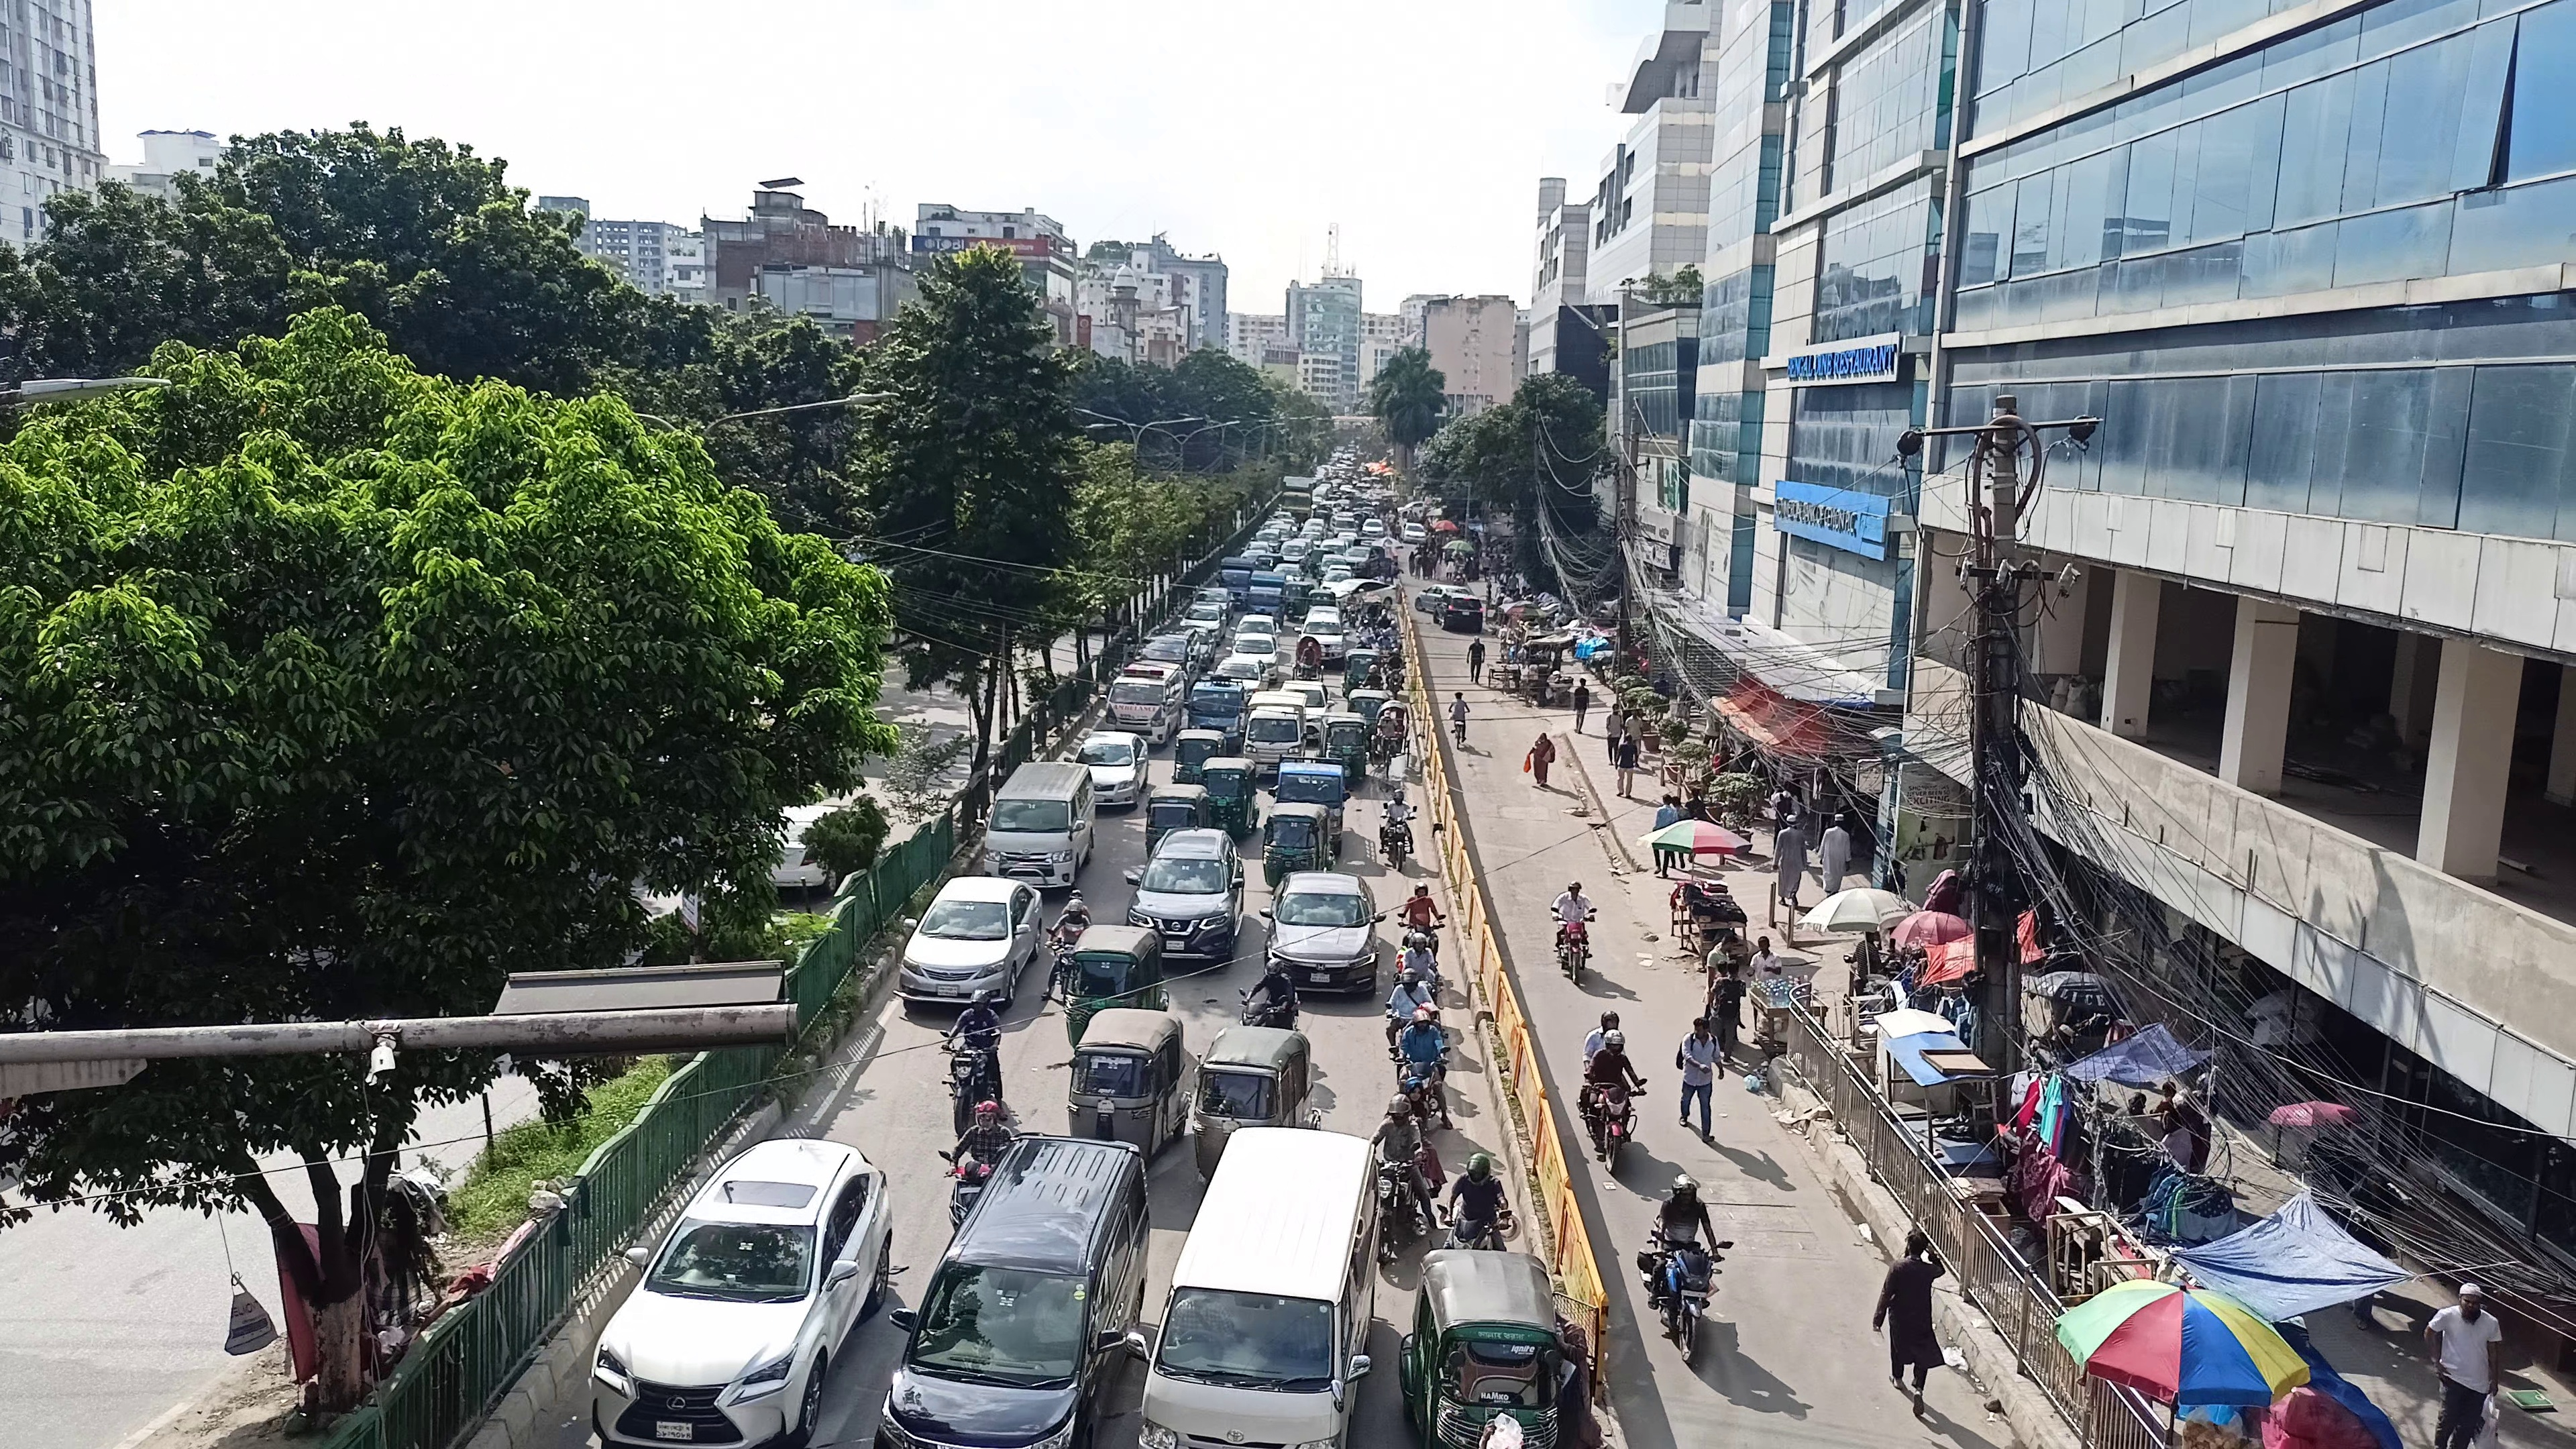
\includegraphics[width=0.28\textwidth]{7.jpg}
    \caption{CCTV footage} % Caption should work fine here
    \label{fig:f1} % Optional: Adding label for reference
\end{wrapfigure}

In this method, the real-time video experiment subsystem is designed to report adaptively to fickleness in traffic density on the road, sudden events, or violations, thereby assuring an effective traffic system. By applying neural networks, the system obtains the capacity for the conclusion, qualifying it to define and adapt to formerly unseen conditions that may arise in real-world urban traffic environments on the road.

\subsection{Object Detection}
The machine learning model is closely trained to attain a high level of exactness in identifying and classifying vehicles, emergency vehicles, and passersby (see Fig. \ref{fig:f2}). This method engages in employing state-of-the-art deep learning algorithms, including convolutional neural networks (CNNs), as well as expanding training datasets to assure strong performance under various situations. These include changes in weather (e.g., heavy rainfall, fog), illumination (e.g., nighttime versus daytime), and traffic consistency (e.g., congested versus free-flowing conditions). The training method is extensive, surrounding challenging scenarios to ensure the model's toughness and reliability. Object identification exactness is elementary to the overall proficiency and reliability of the traffic control system, as it directly influences the decision-making method. 

\begin{figure}
    \centering
    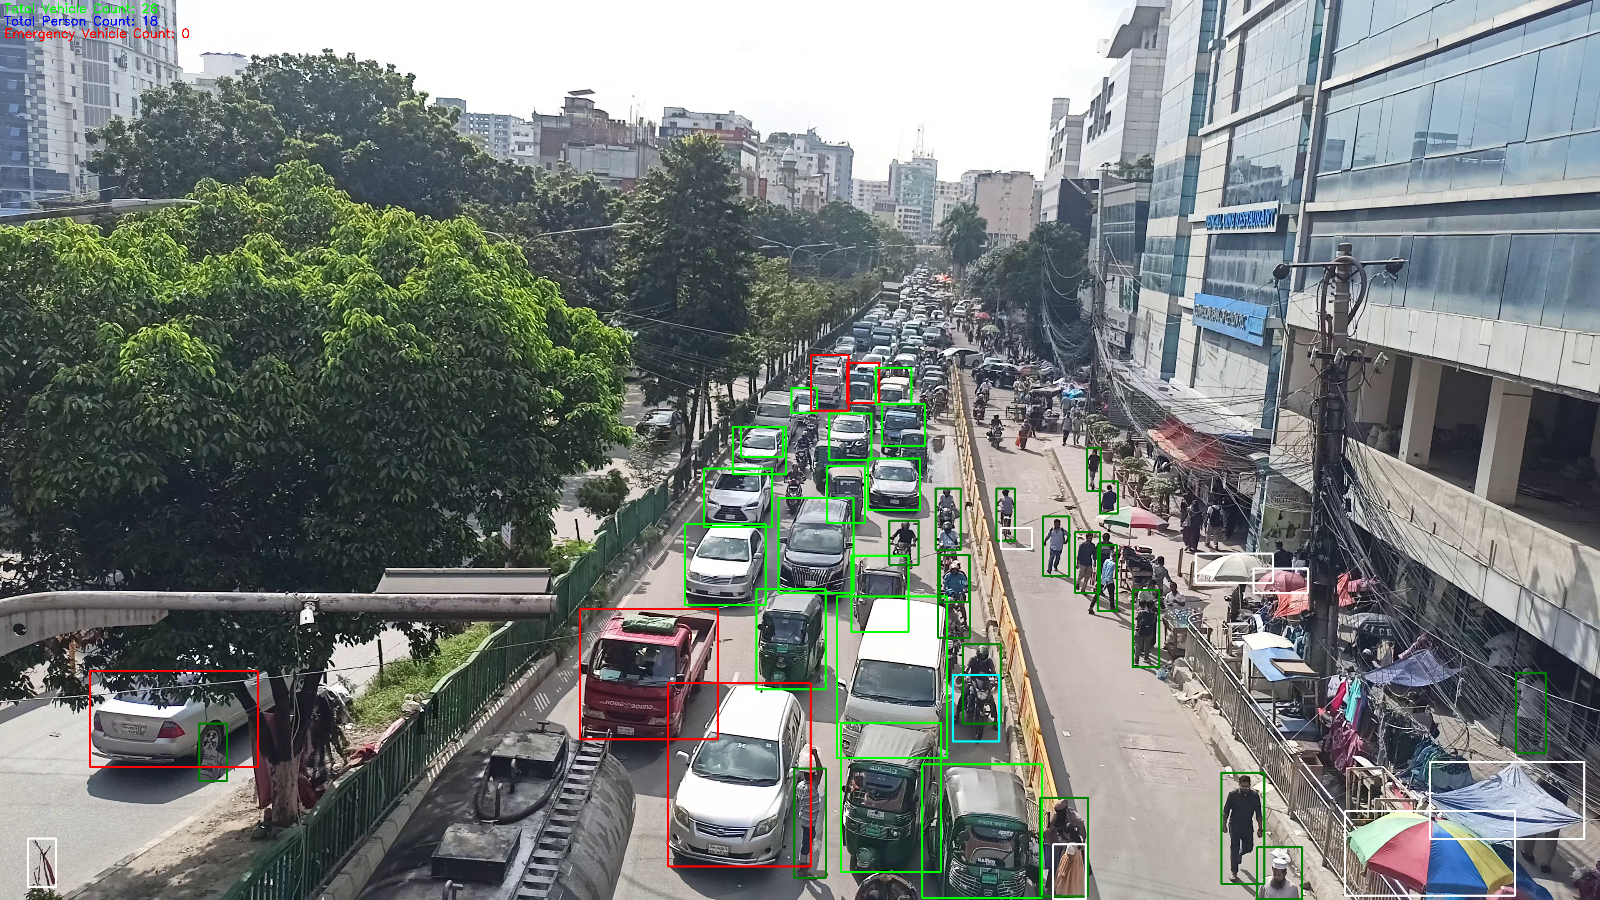
\includegraphics[width=0.5\textwidth]{8.png} % Takes the entire width of the text
    \caption{Using machine learning for vehicle and pedestrian detection.}
    \label{fig:f2}
\end{figure}

Besides, the model endures etesian retraining and optimization, assembling new data to adapt to express urban traffic situations and to improve its fateful abilities over time.

\subsection{Emergency Vehicle Handling}

Based on the identification of an emergency vehicle on the road, such as an ambulance or fire truck that needs an emergency urgent on the road, the process autonomously and immediately opens as soon as possible. The resembling traffic lane to hurrys the passage of the emergency responder on the road. The method sustains the lane’s open status until the emergency vehicle has cleared every section. In those scenarios engaging multiple emergency vehicles, the process adheres to a priority-based ranking mechanism,
Assuring that each emergency vehicle on the road is benefited serially while maintaining an organized flow on the road of each vehicle. This feature is tough for reducing reaction times and is directly integrated with emergency services to improve adjustments. The method’s capability to notice different types of emergency vehicles on the road, combined with its progressive prioritization capabilities on the road, allows for optimal traffic management during troublesome conditions, Finally contributing to public safety and Their fast movement.  Additionally, by interfacing with real-time databases using technology maintained by emergency services on the road, the process can fathom the coming of emergency vehicles on which lane and preemptively optimize traffic flow to create a clear path for the people on the road and draw a relief situation on them.

\subsection{Traffic Flow Optimization}
For non-emergency traffic, the system implements a 
\textbf{*Weighted Job First (WJF)*} scheduling algorithm to determine which lane should be opened next. The WJF algorithm assigns priority weights to each lane based on factors such as the number of vehicles present, pedestrian activity (see Fig. \ref{fig:f3}), and the elapsed time since the lane was last opened. By dynamically adjusting lane priorities,
\begin{wrapfigure}{l}{0.3\textwidth}
    \centering
    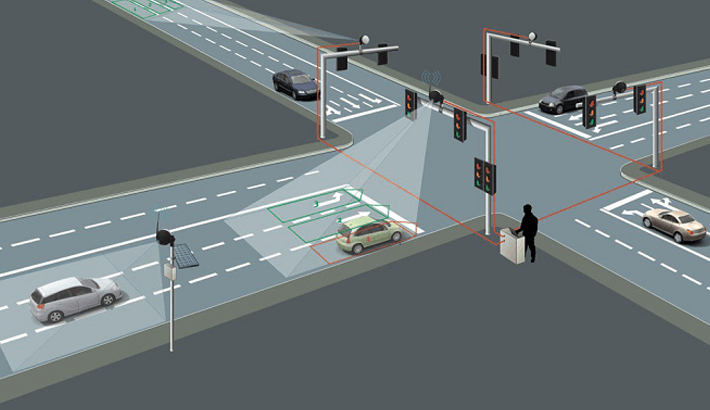
\includegraphics[width=0.28\textwidth]{2_.jpg}
    \caption{Traffic flow determination} % Caption should work fine here
    \label{fig:f3} % Optional: Adding label for reference
\end{wrapfigure}
the system minimizes congestion and ensures equitable access to all lanes, thus avoiding the risk of traffic starvation. Moreover, the system utilizes contextual data such as time of day, historical traffic patterns, and known road closures to optimize the decision-making process. For instance, during rush hours, lanes with higher vehicle densities receive greater weights to alleviate congestion. The system is equipped with predictive capabilities that use machine learning to forecast traffic patterns based on historical data, enabling proactive management that ensures continuous and balanced traffic flow, even during periods of fluctuating demand.

\subsection{Minimum and Maximum Lane Duration}
In the issue of maintaining traffic congestion, the experimental of minimum and maximum time limits for each lane's on-road open state is a tough view of the methodology. These limits are automatically adjusted based on real-time traffic situations and calculated demand. By ensuring that each lane on the road remains open for at least the minimum duration while never exceeding the maximum, the system maintains a balance between proficiency and equity in the traffic management system on the road. This approach relieves the risk of traffic buildup in less-favored lanes while assuring that high-traffic lanes take enough attention during peak periods of rush time. The model also analyses fateful analytics material that leverages historical data to fine-tune lane timings on the road. This assures optimal lane management of vehicles, reducing both the likelihood of traffic bottlenecks and the risk of enhanced waiting times for any single lane while another is starving of vehicles. The adaptive nature of this element also allows for the confirmation of passersby needs, integrating passerby crossing times into the algorithm to promote road safety for all users and travelers.

\subsection{Hardware Signal Integration}

\begin{wrapfigure}{r}{0.4\textwidth}  % Adjust 0.9 for the wrapping width
    \centering
    \begin{minipage}[b]{0.16\textwidth}
        \centering
        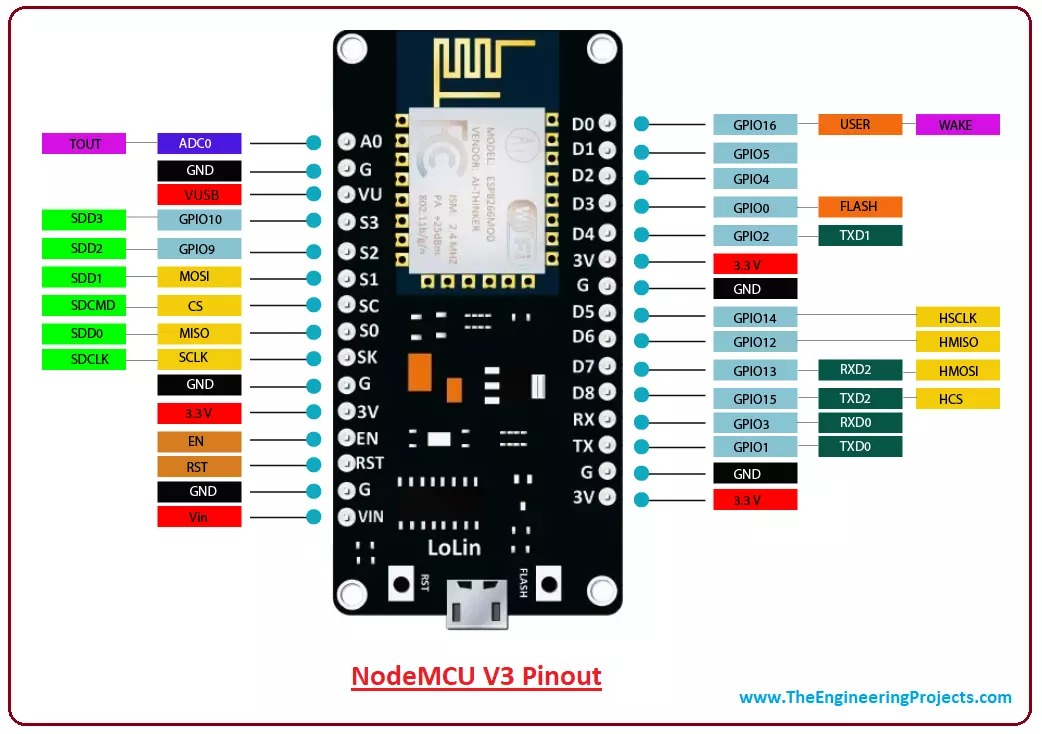
\includegraphics[width=\textwidth]{3.jpeg}
    \end{minipage}
    \hspace{0.01\textwidth} % Adds space between images
    \begin{minipage}[b]{0.16\textwidth}
        \centering
        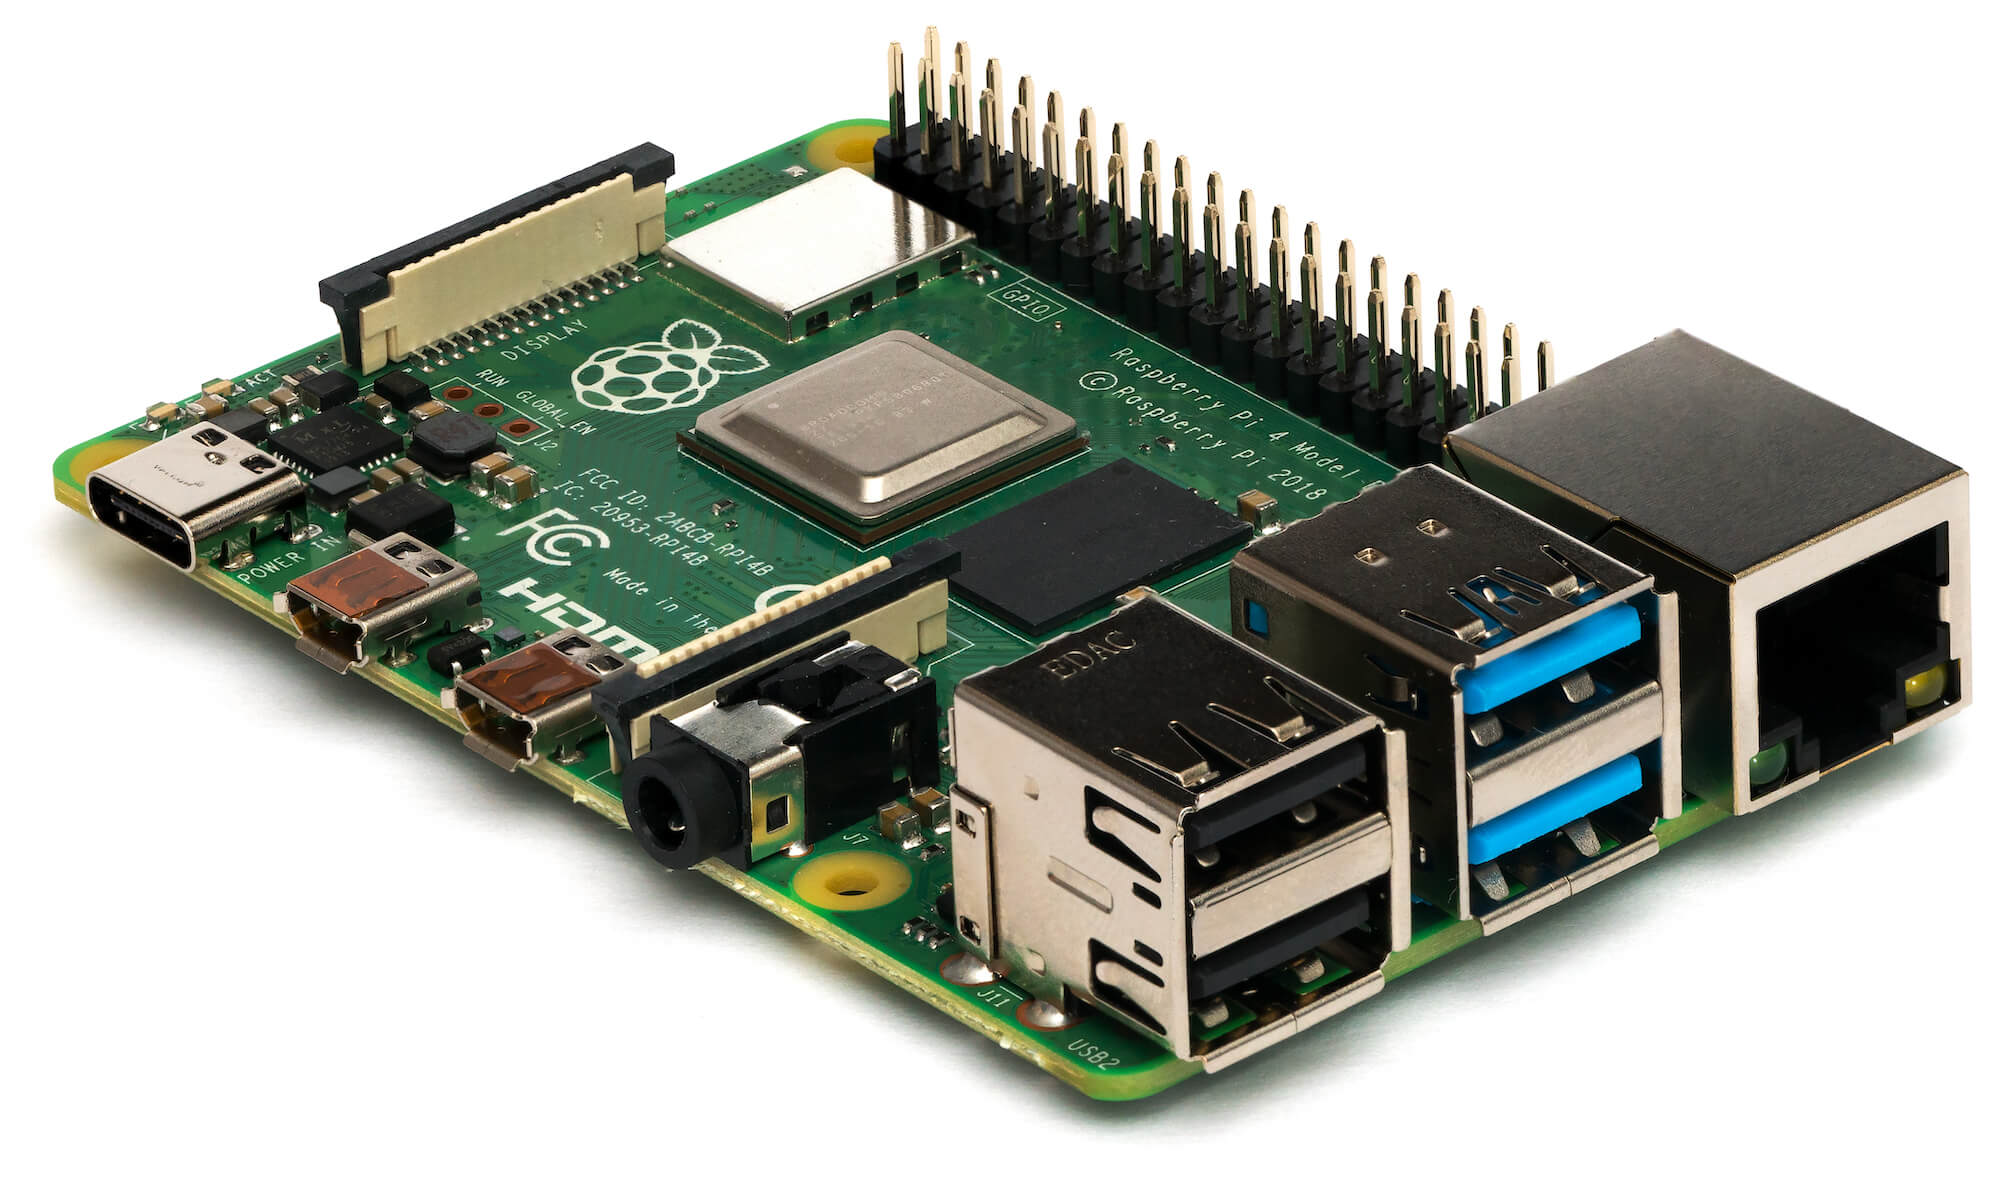
\includegraphics[width=\textwidth]{4.jpg}
    \end{minipage}
    \hspace{0.01\textwidth}
    \begin{minipage}[b]{0.16\textwidth}
        \centering
        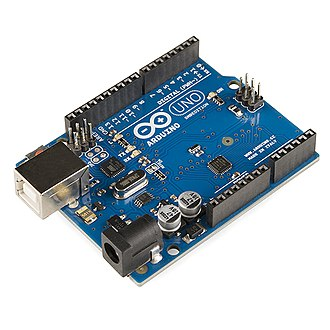
\includegraphics[width=\textwidth]{5.jpg}
    \end{minipage}
    \caption{Microcontrollers}
    \label{fig:f4}
\end{wrapfigure}

Upon determining which lane to open or close, the system transmits a signal to the hardware controllers—typically microcontrollers (see Fig. \ref{fig:f4}) such as Arduino, Raspberry Pi, or NodeMCU—which manage the physical traffic lights. The use of resilient microcontrollers allows for precise and reliable control of traffic lights \citep{clar:a12} \citep{clar:a13}, with the added capability of scalability to multiple intersections across a city.
% \begin{wrapfigure}{r}{0.2\textwidth}
%     \centering
%     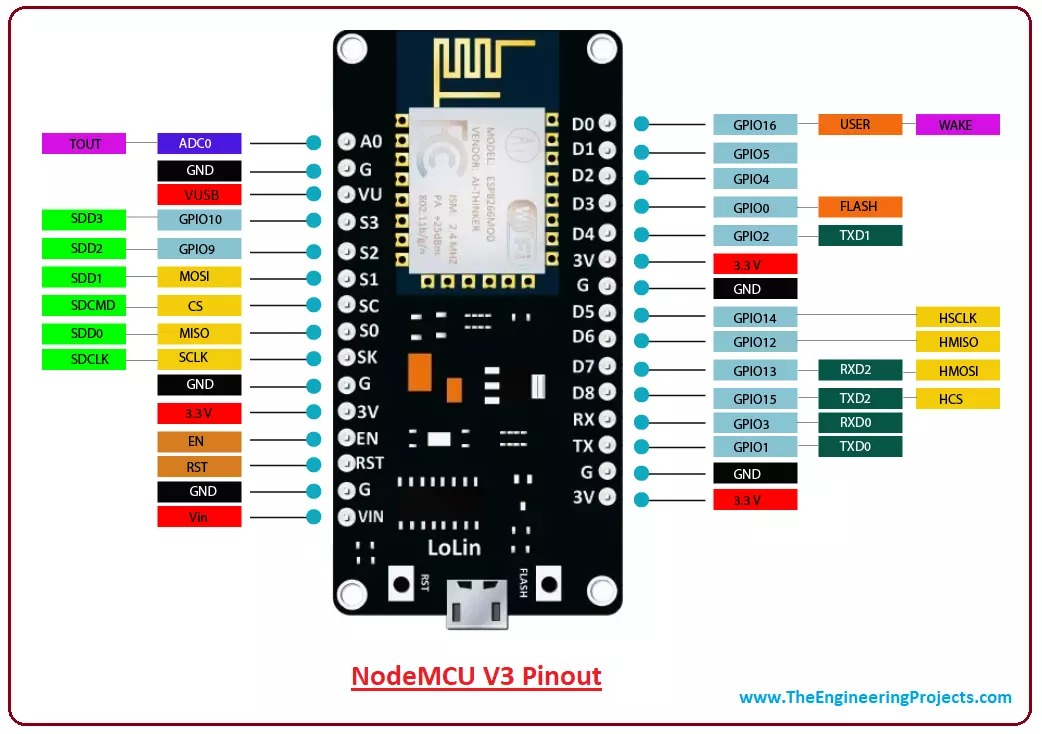
\includegraphics[width=0.2\textwidth]{3.jpeg}
%     \caption{NodeMCU}
%     \label{fig:wrap1}
% \end{wrapfigure}
These microcontrollers serve as the interface between the machine learning control algorithms and the physical traffic signal infrastructure.

% \begin{figure}[H]
%     \centering
%     \begin{minipage}{0.5\textwidth}
%         \centering
%         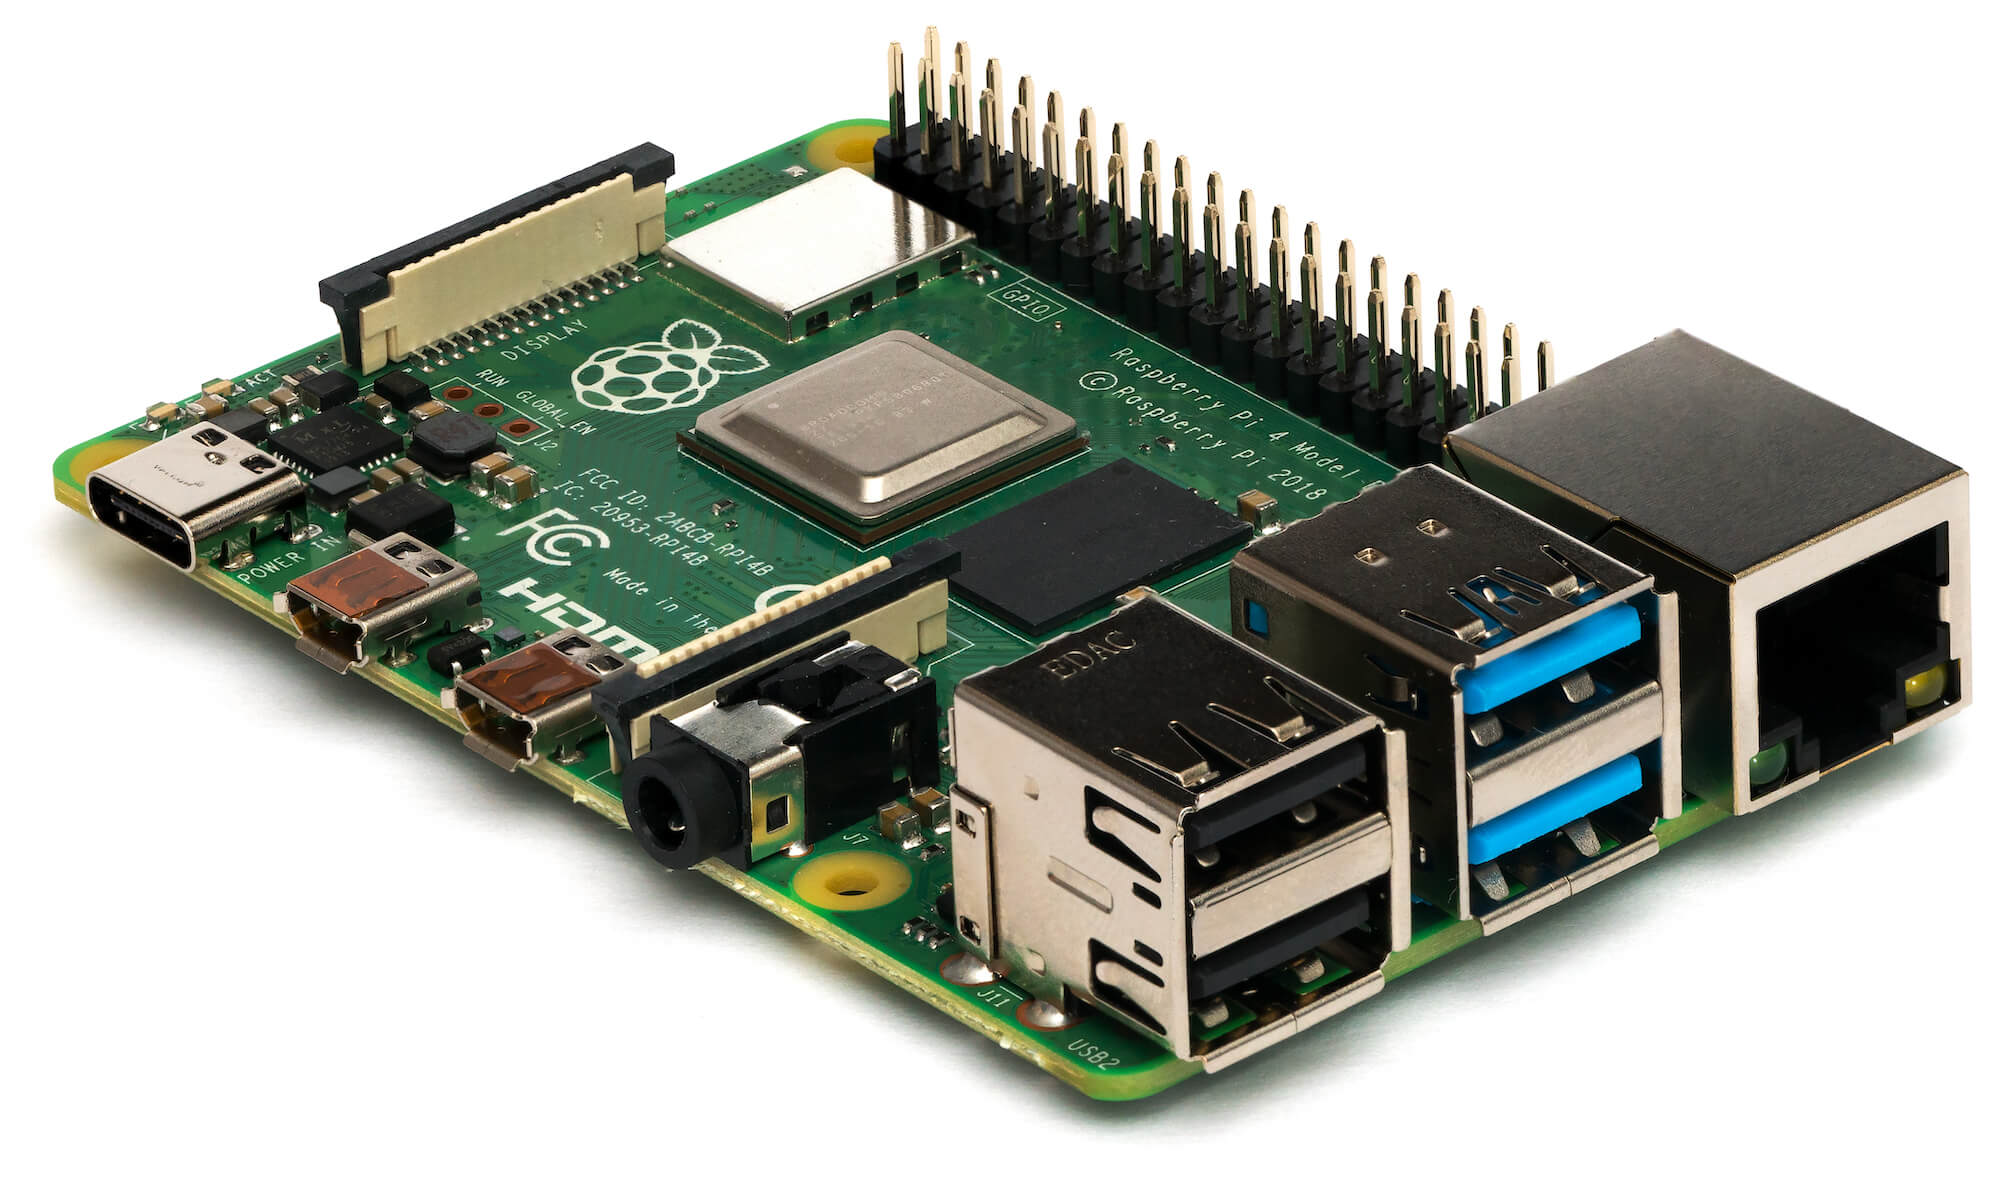
\includegraphics[width=0.6\textwidth]{4.jpg}
%         \caption{Raspberry Pi}
%         \label{fig:wrap2}
%     \end{minipage}%
%     \hfill % Add some spacing between images
%     \begin{minipage}{0.4\textwidth}
%         \centering
%         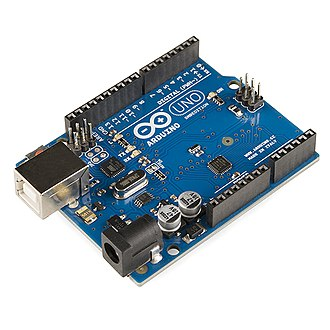
\includegraphics[width=0.6\textwidth]{5.jpg}
%         \caption{Arduino}
%         \label{fig:wrap3}
%     \end{minipage}
% \end{figure}

This facilitates the deployment of an intelligent traffic management system on a broader scale. To ensure robustness, the hardware controllers are equipped with fail-safe mechanisms to maintain proper traffic light operation even in the event of hardware or software malfunctions.


\subsection[]{Apply Algorithm}

The traffic control system operates within a continuous feedback loop, 
consisting of sequential stages: real-time video analysis, object detection, lane prioritization, and hardware signal activation. This continuous loop structure ensures that traffic control decisions are always informed by the most current data, thereby allowing the system to adapt to sudden changes in traffic conditions, such as accidents or surges in vehicle numbers.  algorithmic control and human expertise.
% \clearpage
% \begin{figure}
%   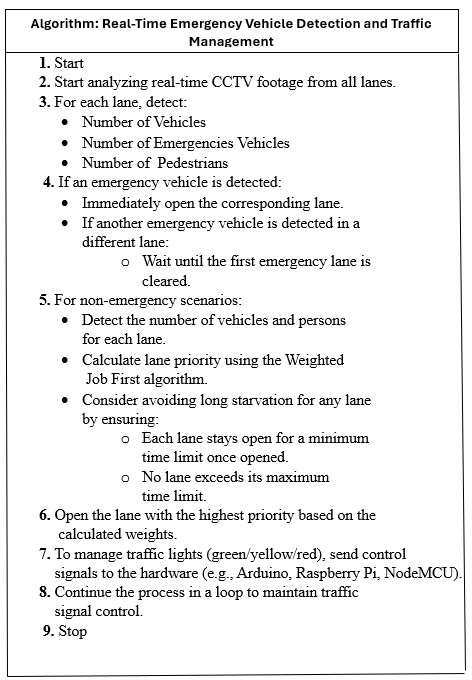
\includegraphics[width=\columnwidth]{10.png}
%   % \caption{Example of a simple single-column figure. Don't put this
%   %   too early in the document since we don't want it to go in the
%   %   first column.}
%   \label{fig:simple}
% \end{figure}
\noindent % Prevent indentation
\begin{minipage}{0.5\textwidth}
    \centering
    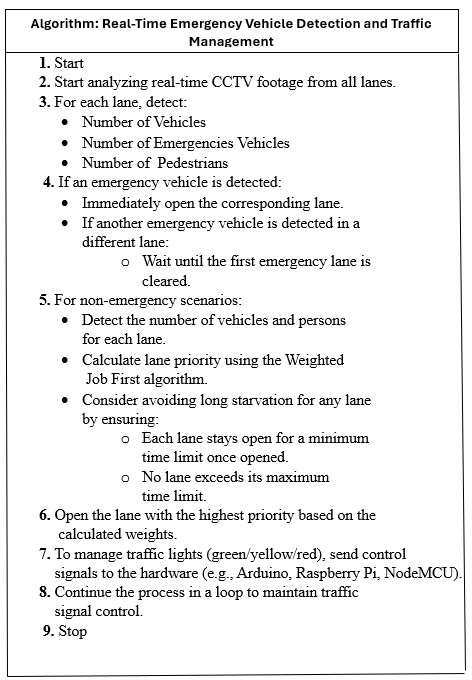
\includegraphics[width=\textwidth]{10.png} % Image takes full width of the 50% column
    \vspace{0.3cm}
    % \captionof{figure}{Pseudo Code}
\end{minipage}%

The loop operates with minimal latency, optimizing system responsiveness and ensuring real-time adaptation to dynamic traffic environments. Furthermore, an embedded feedback mechanism analyzes the outcomes of previous iterations to optimize future decision-making. This iterative learning approach facilitates continuous improvement in traffic control efficiency. An oversight mechanism, supported by anomaly detection algorithms, monitors the loop process for irregularities. If unusual patterns are detected—such as sustained congestion in a particular lane—alerts are generated for human operators, allowing for manual intervention when automated responses are insufficient. By integrating human oversight into the system's automated processes, the methodology maintains a balance between
% \noindent % Prevent indentation
% \begin{minipage}{0.5\textwidth}
%     \centering
%     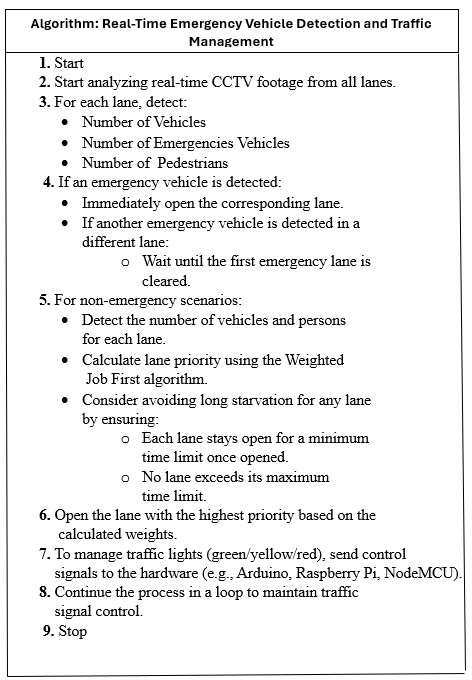
\includegraphics[width=\textwidth]{10.png} % Image takes full width of the 50% column
%     \captionof{figure}{Pseudo Code}
% \end{minipage}%


\subsection{Signal Control}
To control the traffic congestion on the road the process can be manually stopped or paused to simplify scheduled maintenance. At the time of maintenance, all videos that were captured using camera analysis and hardware control methods were safely stopped to obstruct unrevised performances. Maintenance methodologies are structured to allow for serial-wise system updates on the road, including improvements to machine learning models and the integration of new functionalities, without being the reason for stavings to traffic flow at a time on the road. In this paper work prohibitive maintenance includes recalibrating both hardware elements and machine learning models to maintain high quality of exactness and system performance. This recalibration is typically directed during off-peak hours to minimize Breakdown to normal traffic experiments on the road.
% \begin{wrapfigure}{r}{0.5\textwidth}
%     \centering
%     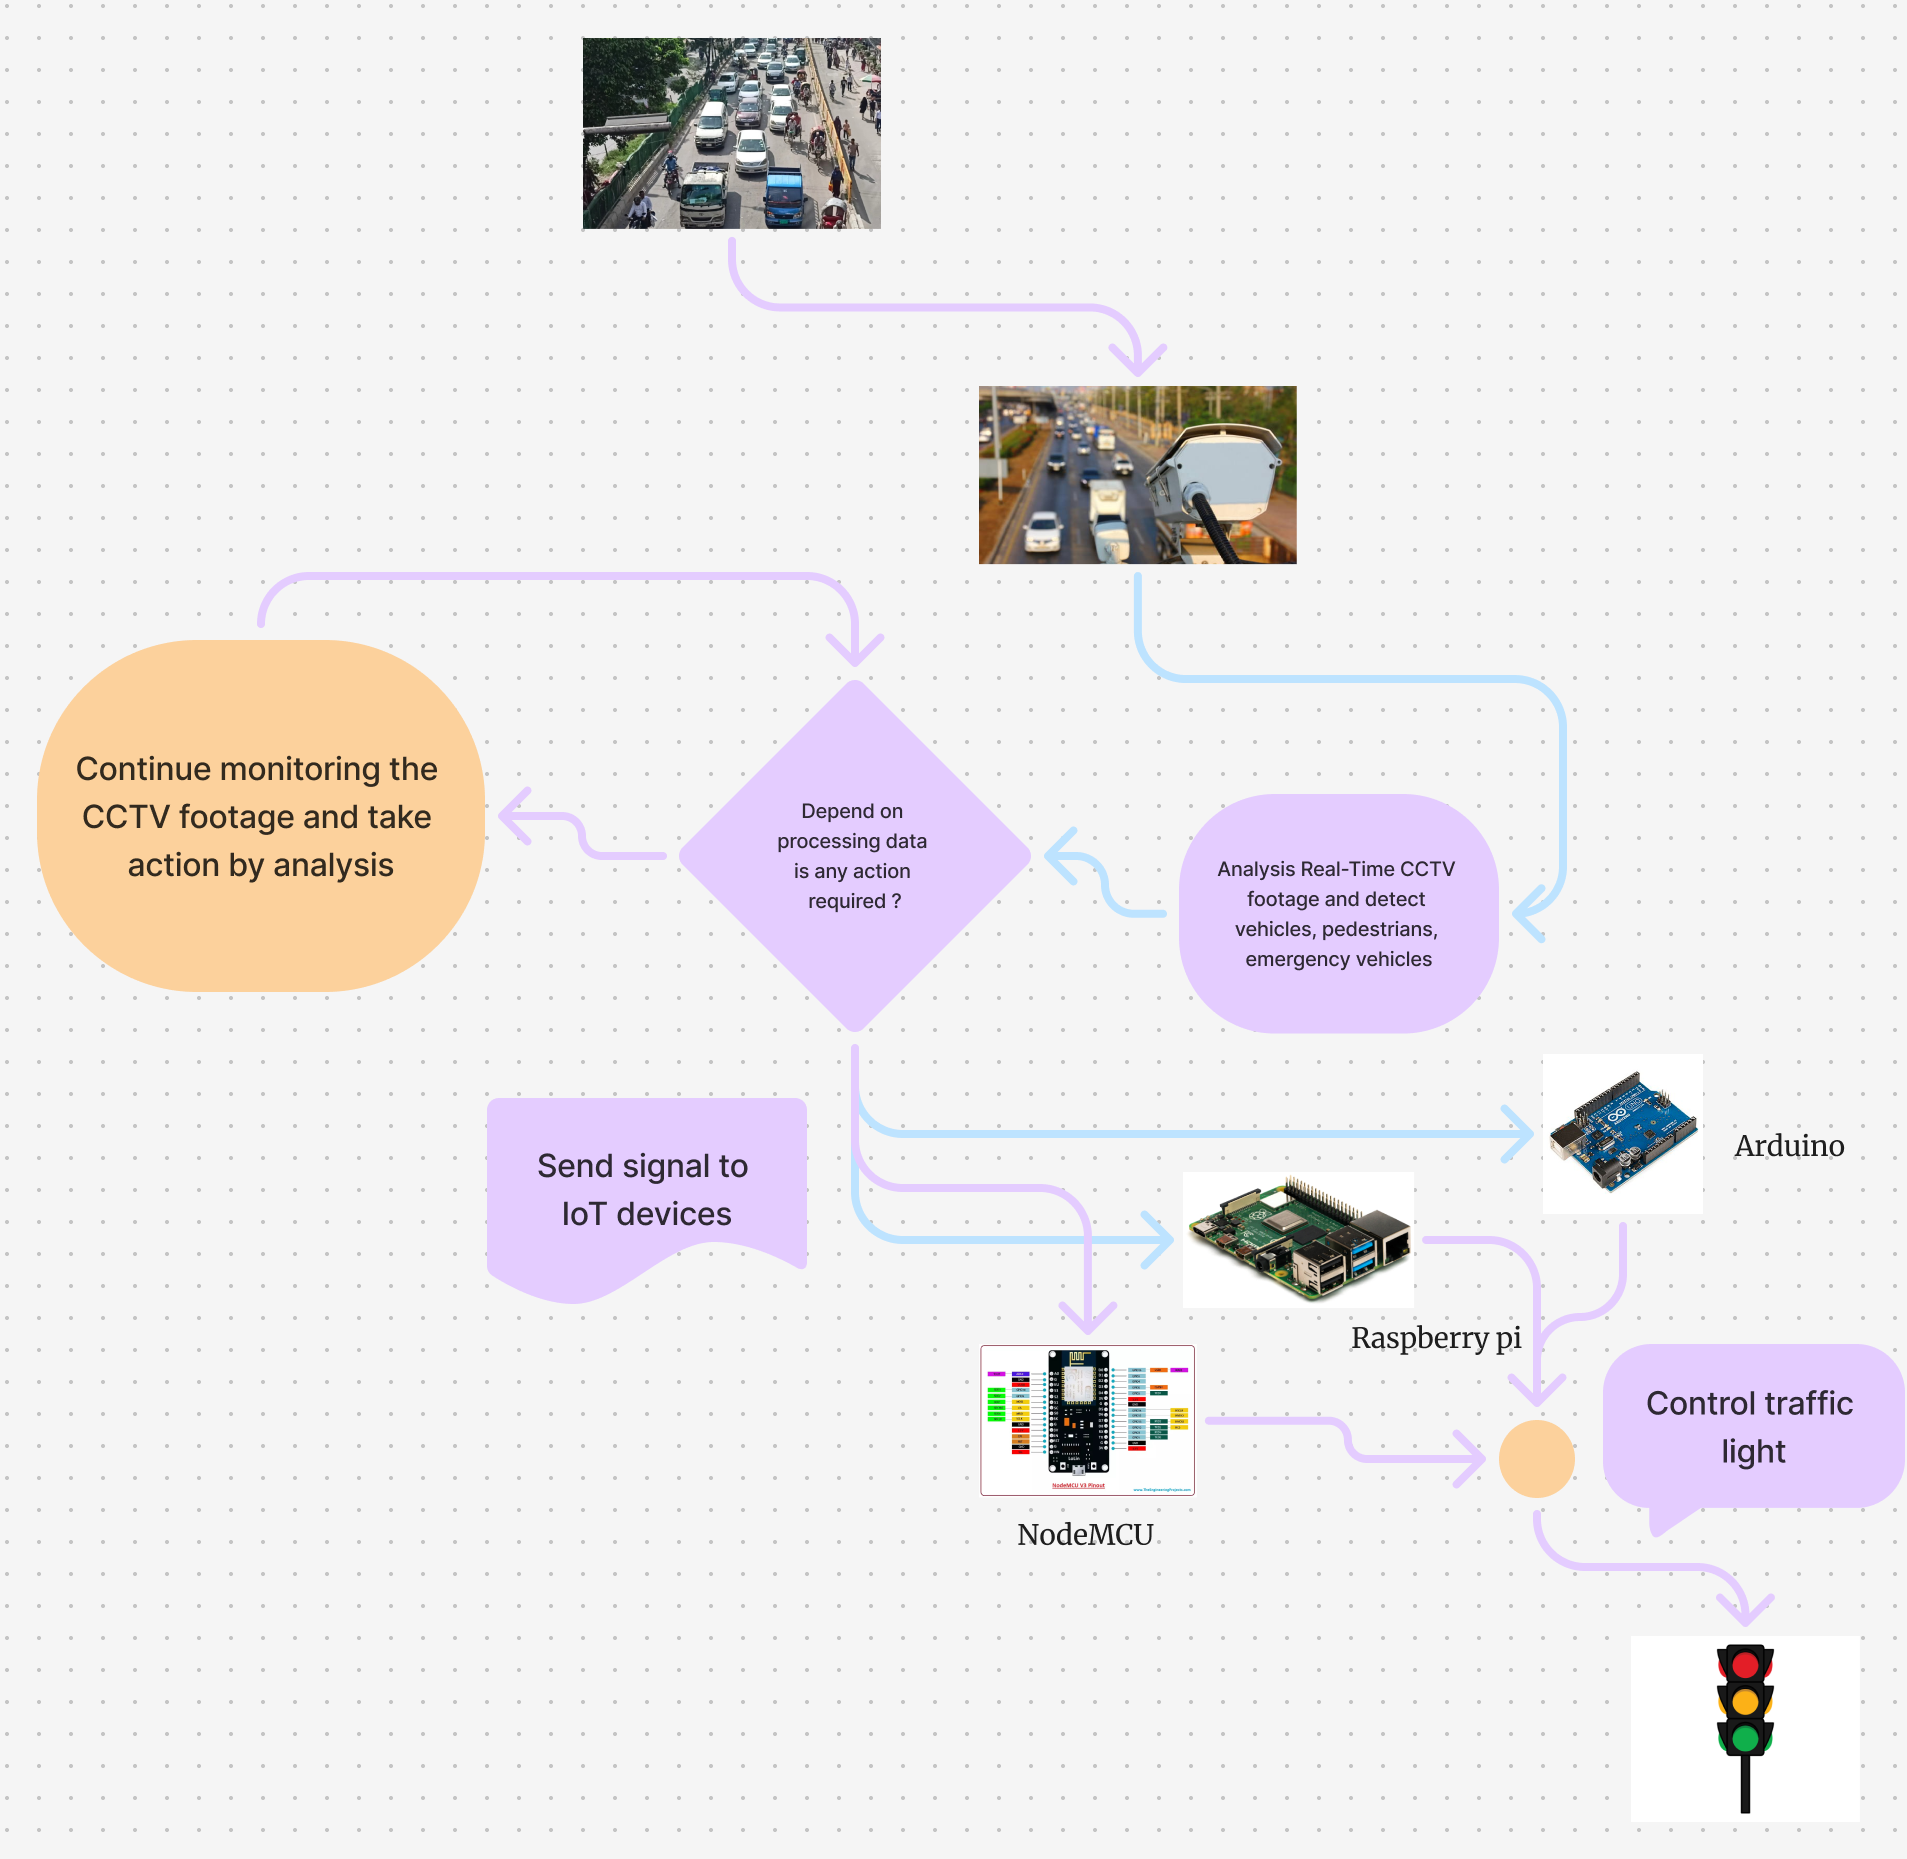
\includegraphics[width=0.5\textwidth]{6_.png}
%     \caption{Workflow}
%     \label{fig:wrap1}
% \end{wrapfigure}
% \begin{figure}
%   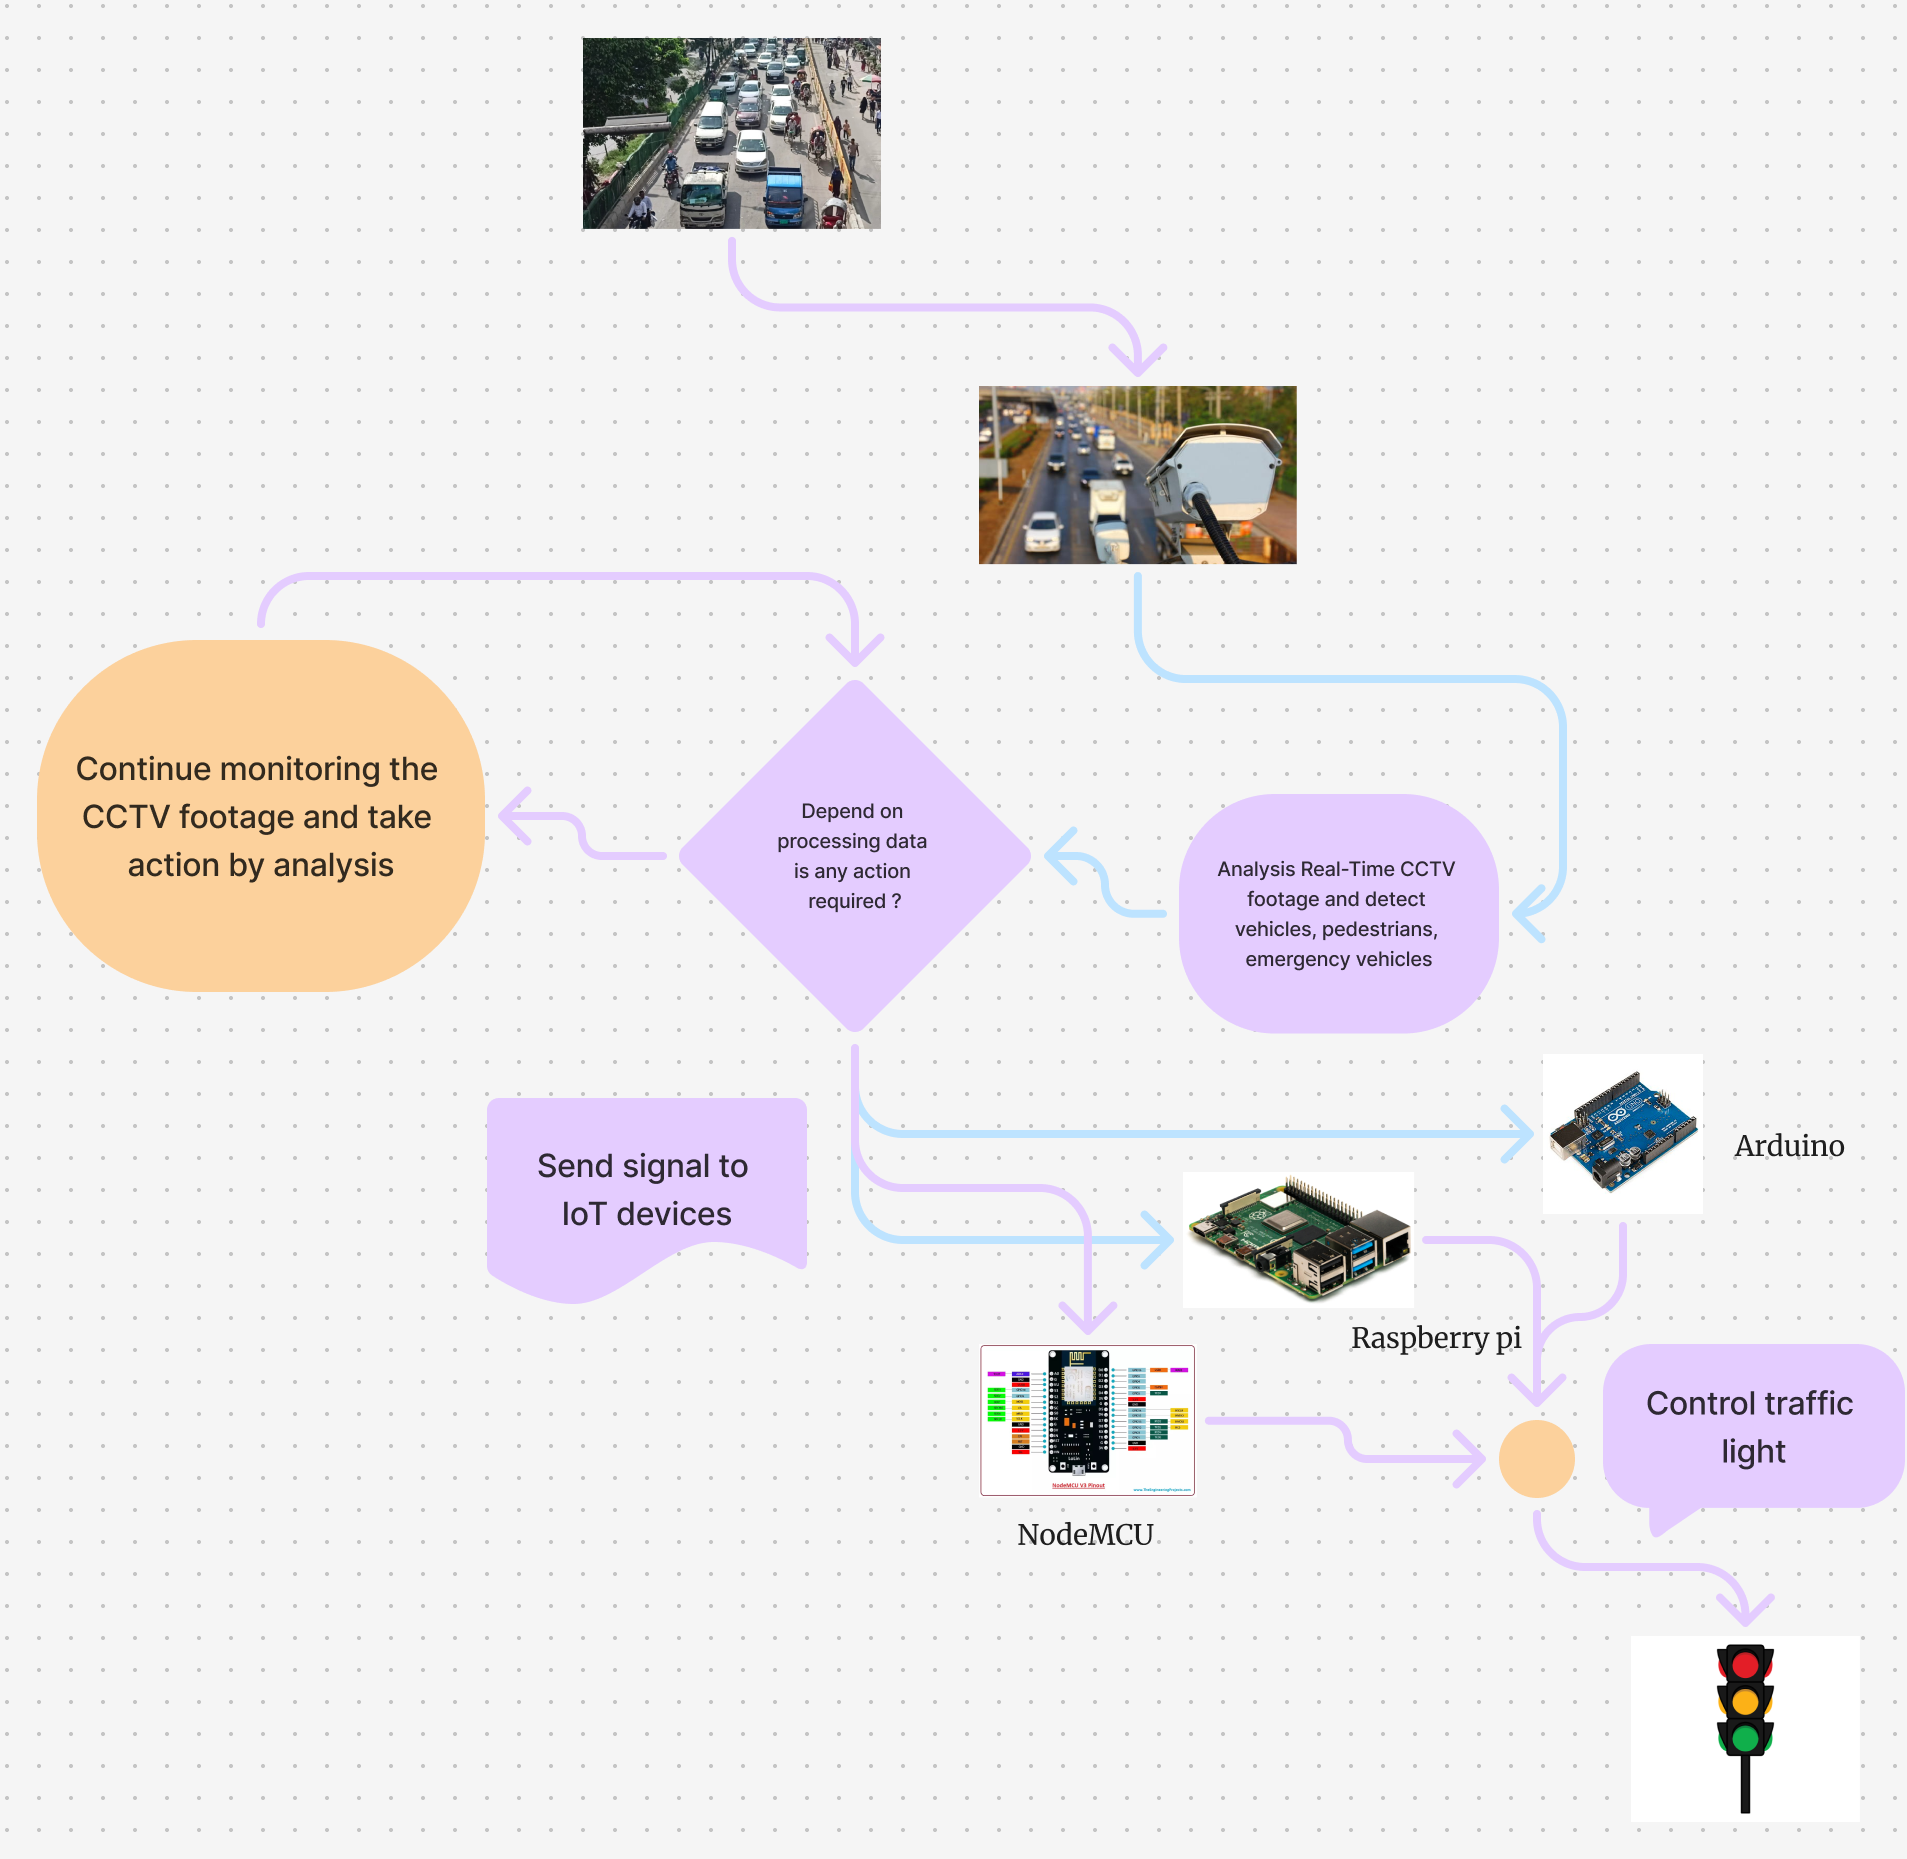
\includegraphics[width=\columnwidth]{6_.png}
%   % \caption{Example of a simple single-column figure. Don't put this
%   %   too early in the document since we don't want it to go in the
%   %   first column.}
%   \label{fig:simple}
% \end{figure}
\vspace{0.5cm}
\begin{minipage}{0.5\textwidth}
    \centering
    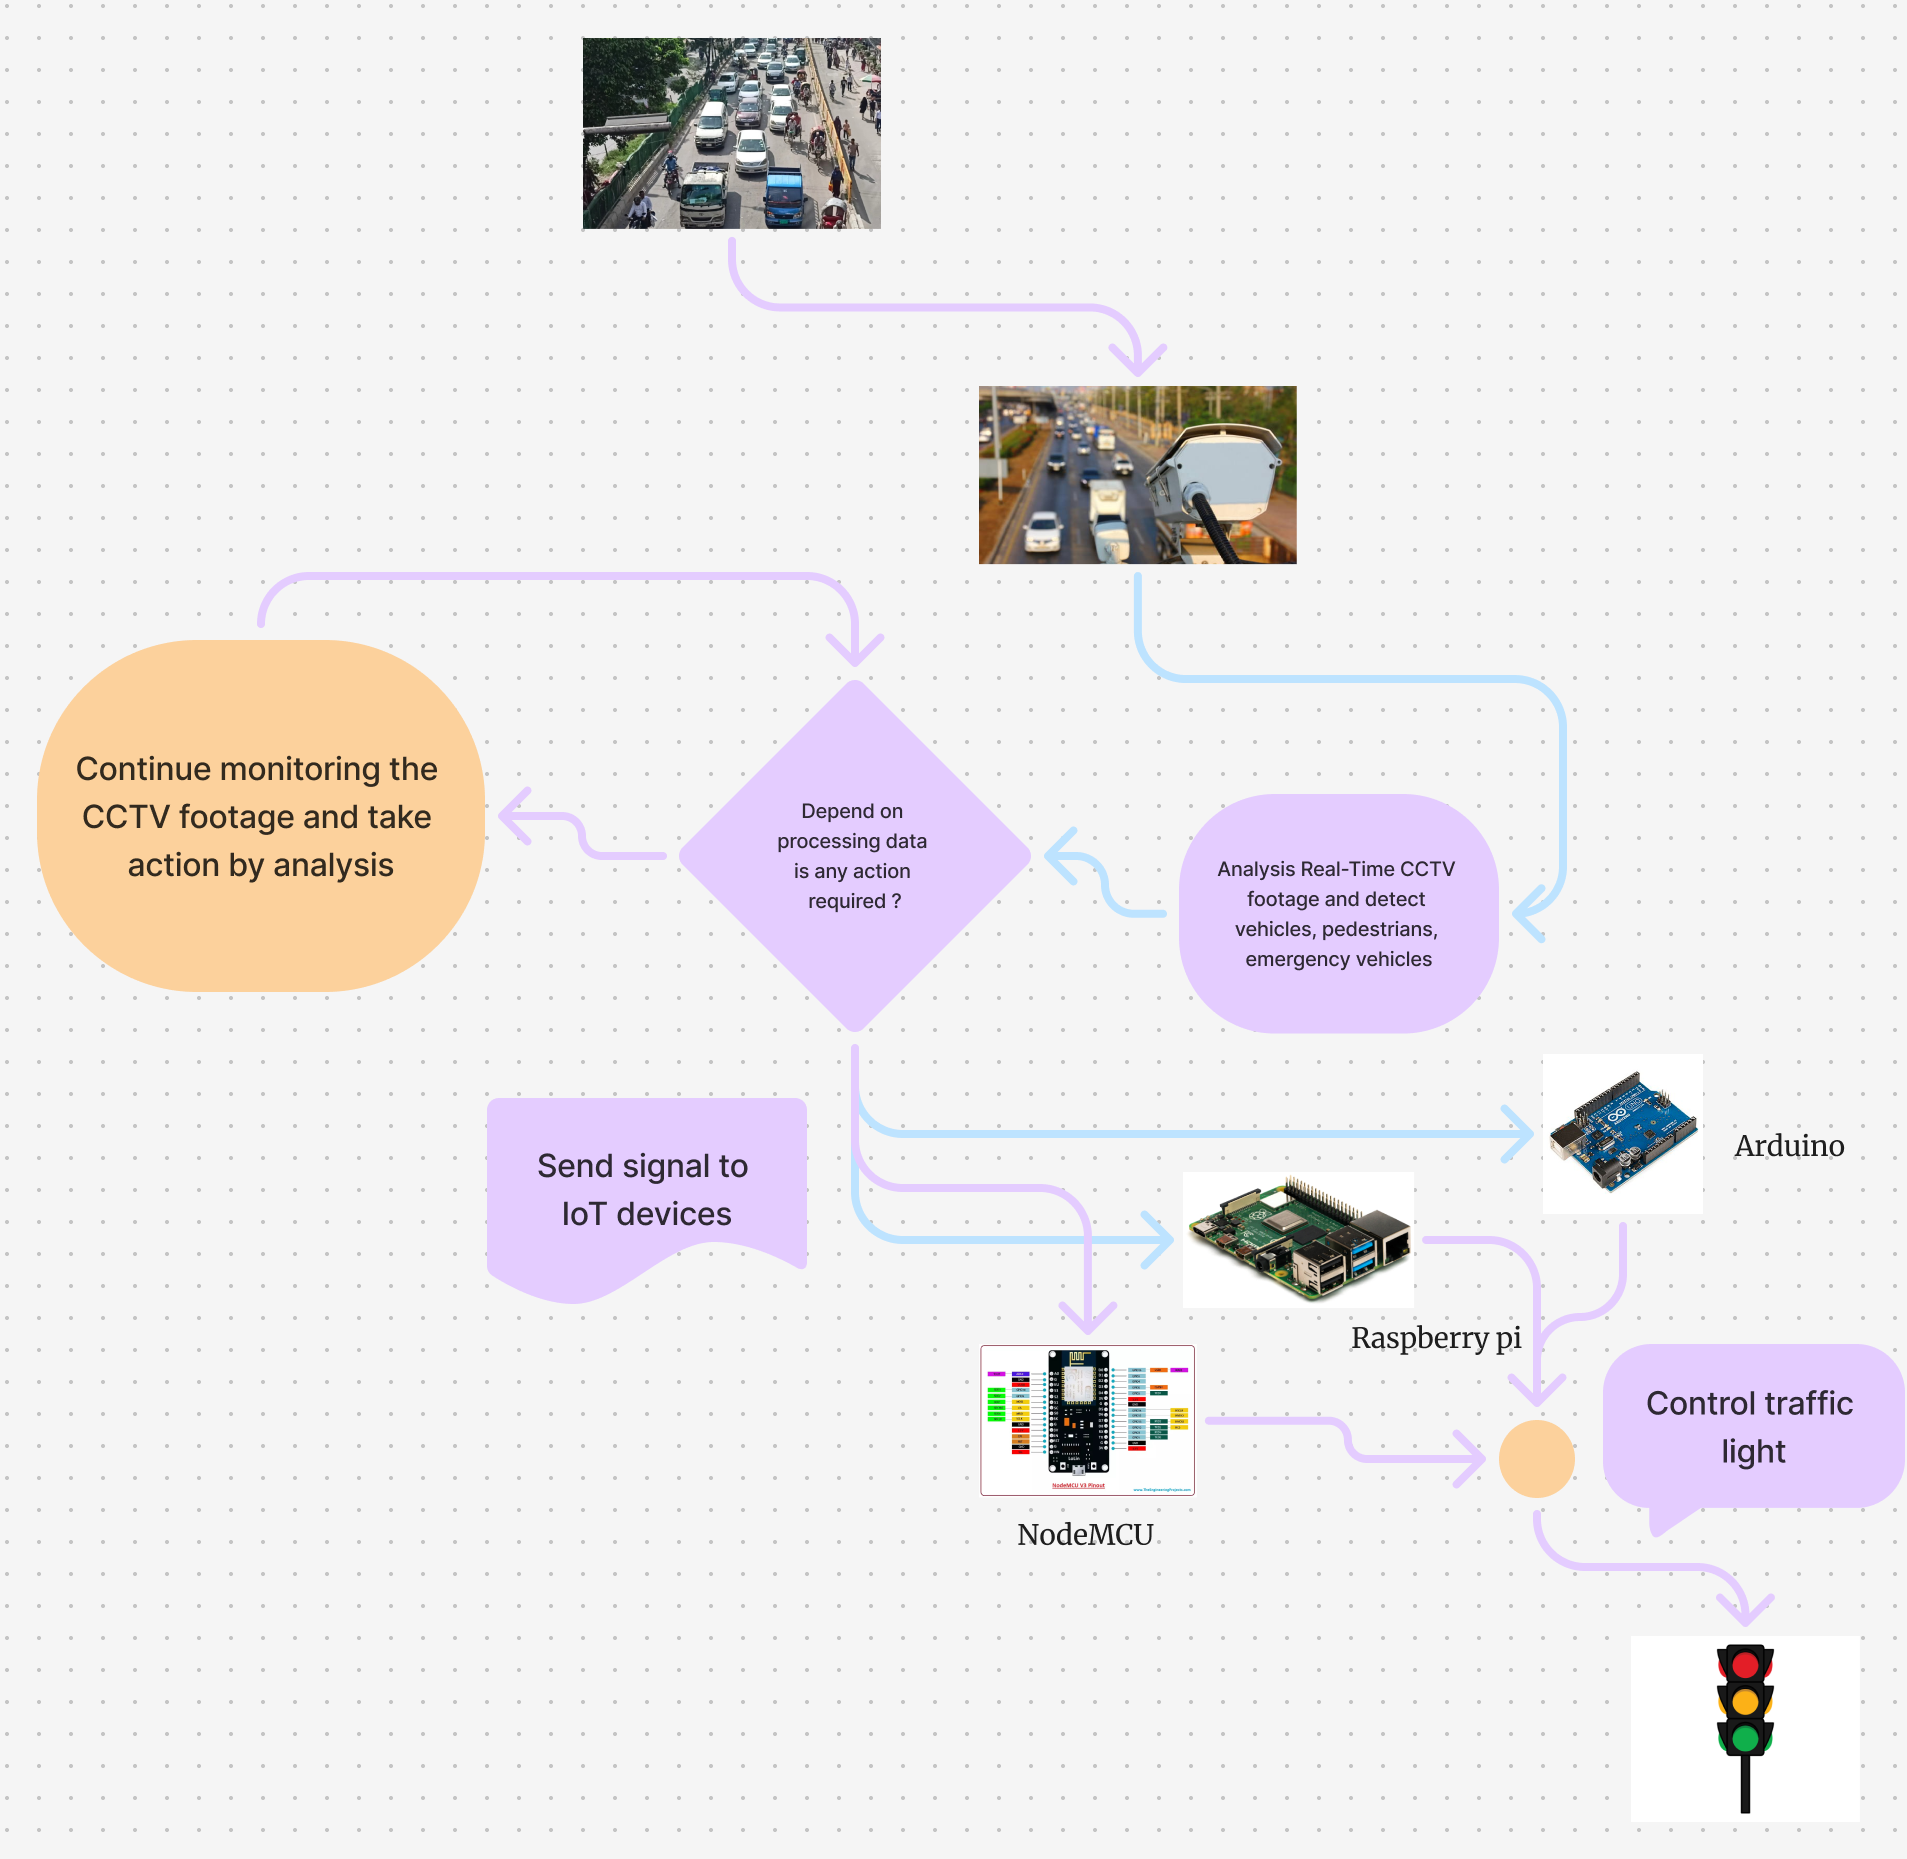
\includegraphics[width=\textwidth]{6_.png}
    \captionof{figure}{Workflow}
\end{minipage}%

Besides, automated diagnostic tools continuously count the health of both software and hardware elements, with real-time alerts created for any detected malfunctions if remain. This proactive maintenance case study not only minimizes downtime but also assures that the process operates at optimal ability at all times, maintaining the integrity and reliability of urban traffic regulation. The excessive mechanisms organized into the process design ensure that even during maintenance activities, messy traffic control functions are conserved, by ensuring continuous service delivery on the road.

\section[]{Result Analysis}
The project will contribute to improvements in traffic efficiency and safety. The results were collected by evaluating key metrics such as average vehicle wait time, emergency vehicle response time, decreased human interaction, and overall traffic flow consistency across multiple intersections in Dhaka and other cities in Bangladesh.

% \noindent % Prevent indentation
\begin{minipage}{0.5\textwidth}
    \centering
    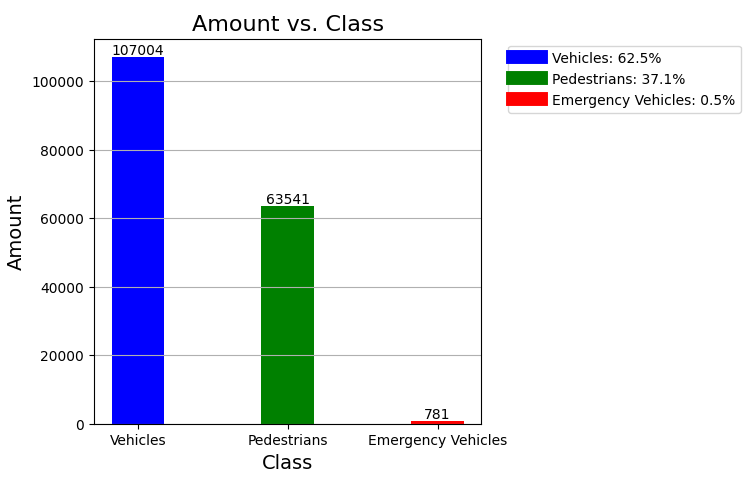
\includegraphics[width=\textwidth]{11.png} % Image takes full width of the 50% column
    \captionof{figure}{Overview of the Annotated Dataset}
    \label{fig:f6}
\end{minipage}%
% \vspace{0.5cm}
We made an ML model for real-time detecting vehicles which have three class vehicles (normal vehicles), emergency vehicles (ambulance, fire truck, etc), and person. We have annotated around 107k vehicles, 63k pedestrians, and for emergency vehicles 781 (see Fig \ref{fig:f6}) and continuously adding more. Now, our model accuracy on 10 epochs is 59 percent, 128 epochs is 68 percent and 256 epochs are 79 percent. We are working to increase it up to 90 percent.


The results and confusion matrix (see Fig. \ref{fig:f7}) of our model after running \textbf{256 epochs}. We previously trained the model using \textbf{100 epochs}, \textbf{128 epochs}, and \textbf{200 epochs}, but found that running the model for \textbf{256 epochs} yielded the best results. 

The confusion matrix shows  that:
\begin{itemize}
    \item The \textbf{Emergency vehicle} class has \textbf{4 instances} that are correctly classified.
    \item The \textbf{Person} class has \textbf{2080 instances} that are correctly classified.
    \item The \textbf{Vehicle} class has \textbf{4111 instances} that are correctly classified.
    \item The \textbf{Background} class has \textbf{1222 instances} that are correctly classified.
\end{itemize}

These results demonstrate a significant improvement over earlier epochs, particularly in distinguishing between vehicles and pedestrians. The final model at 256 epochs exhibits the best performance in classifying the various traffic entities.

The chart demonstrates the distribution of bounding boxes across three categories: vehicles, pedestrians, and emergency vehicles. The model has achieved an overall accuracy of 79\%, which shows significant progress. Here's a breakdown of the observations based on the data:
\begin{figure}
    \centering
    \begin{minipage}{0.5\textwidth}
        \centering
        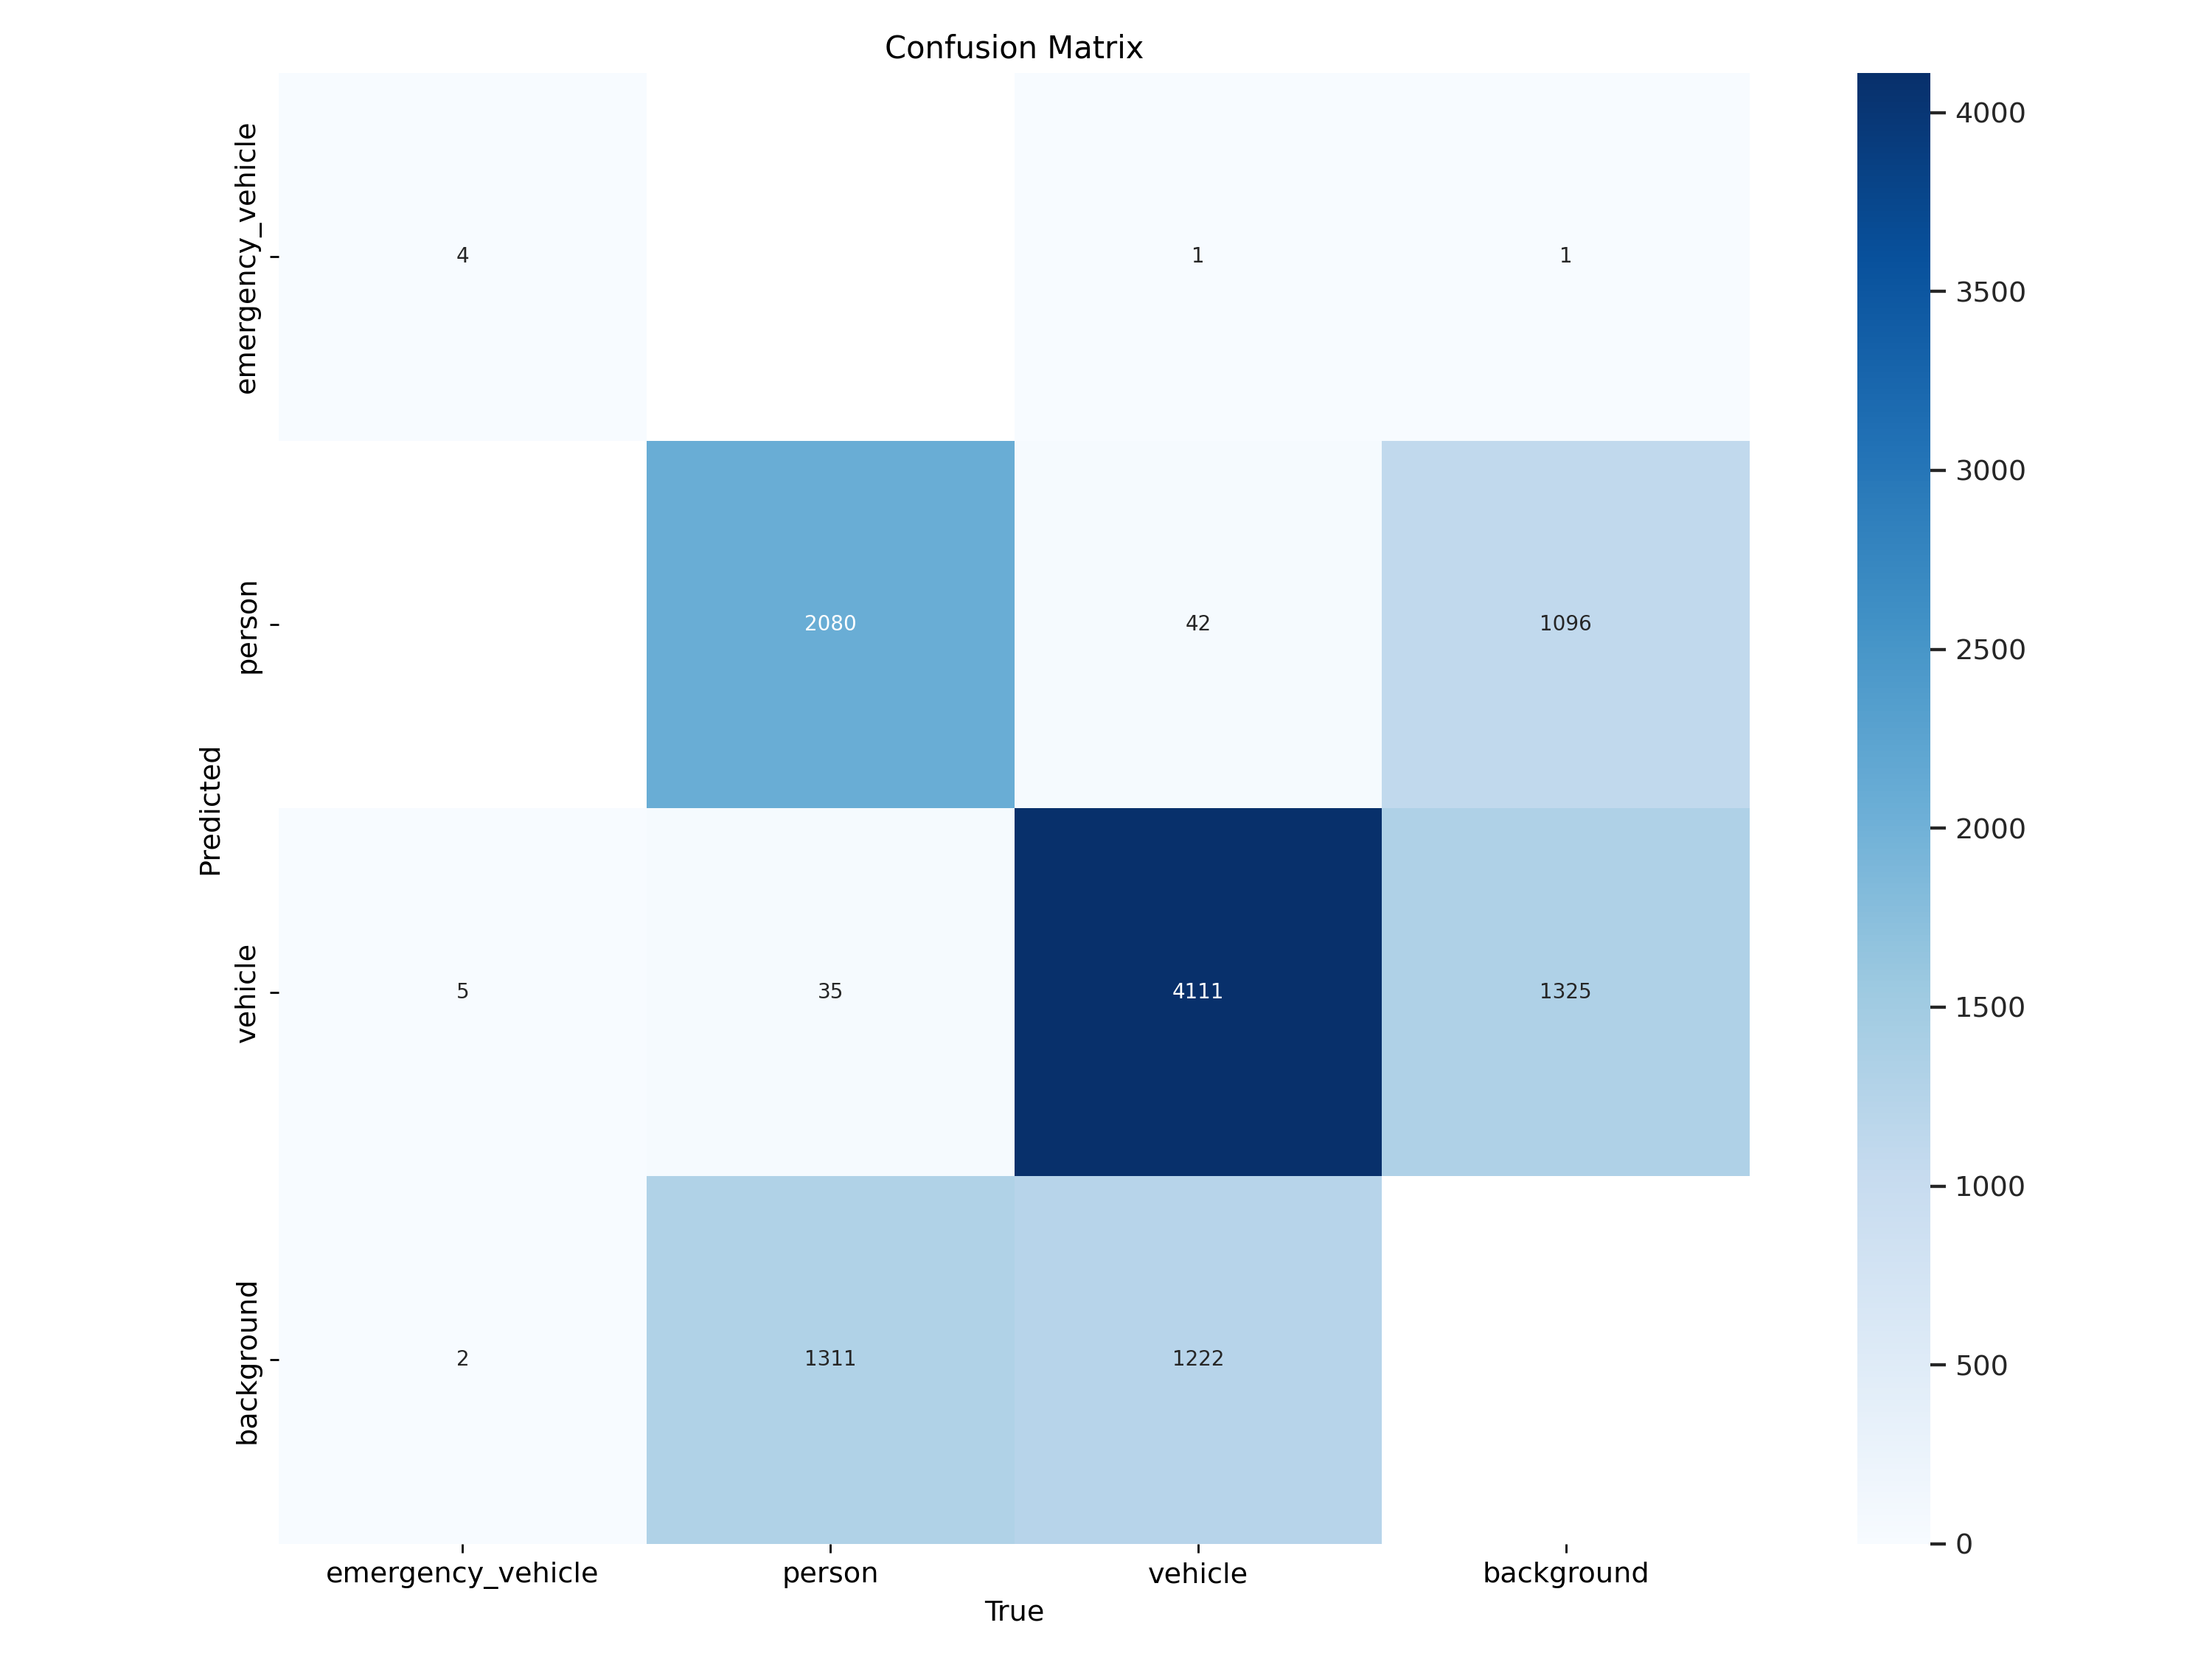
\includegraphics[width=0.9\textwidth]{14.png}
        \caption{Confusion Matrix}
        \label{fig:f7}
    \end{minipage}%
    \hfill % Add some spacing between images
    \begin{minipage}{0.5\textwidth}
        \centering
        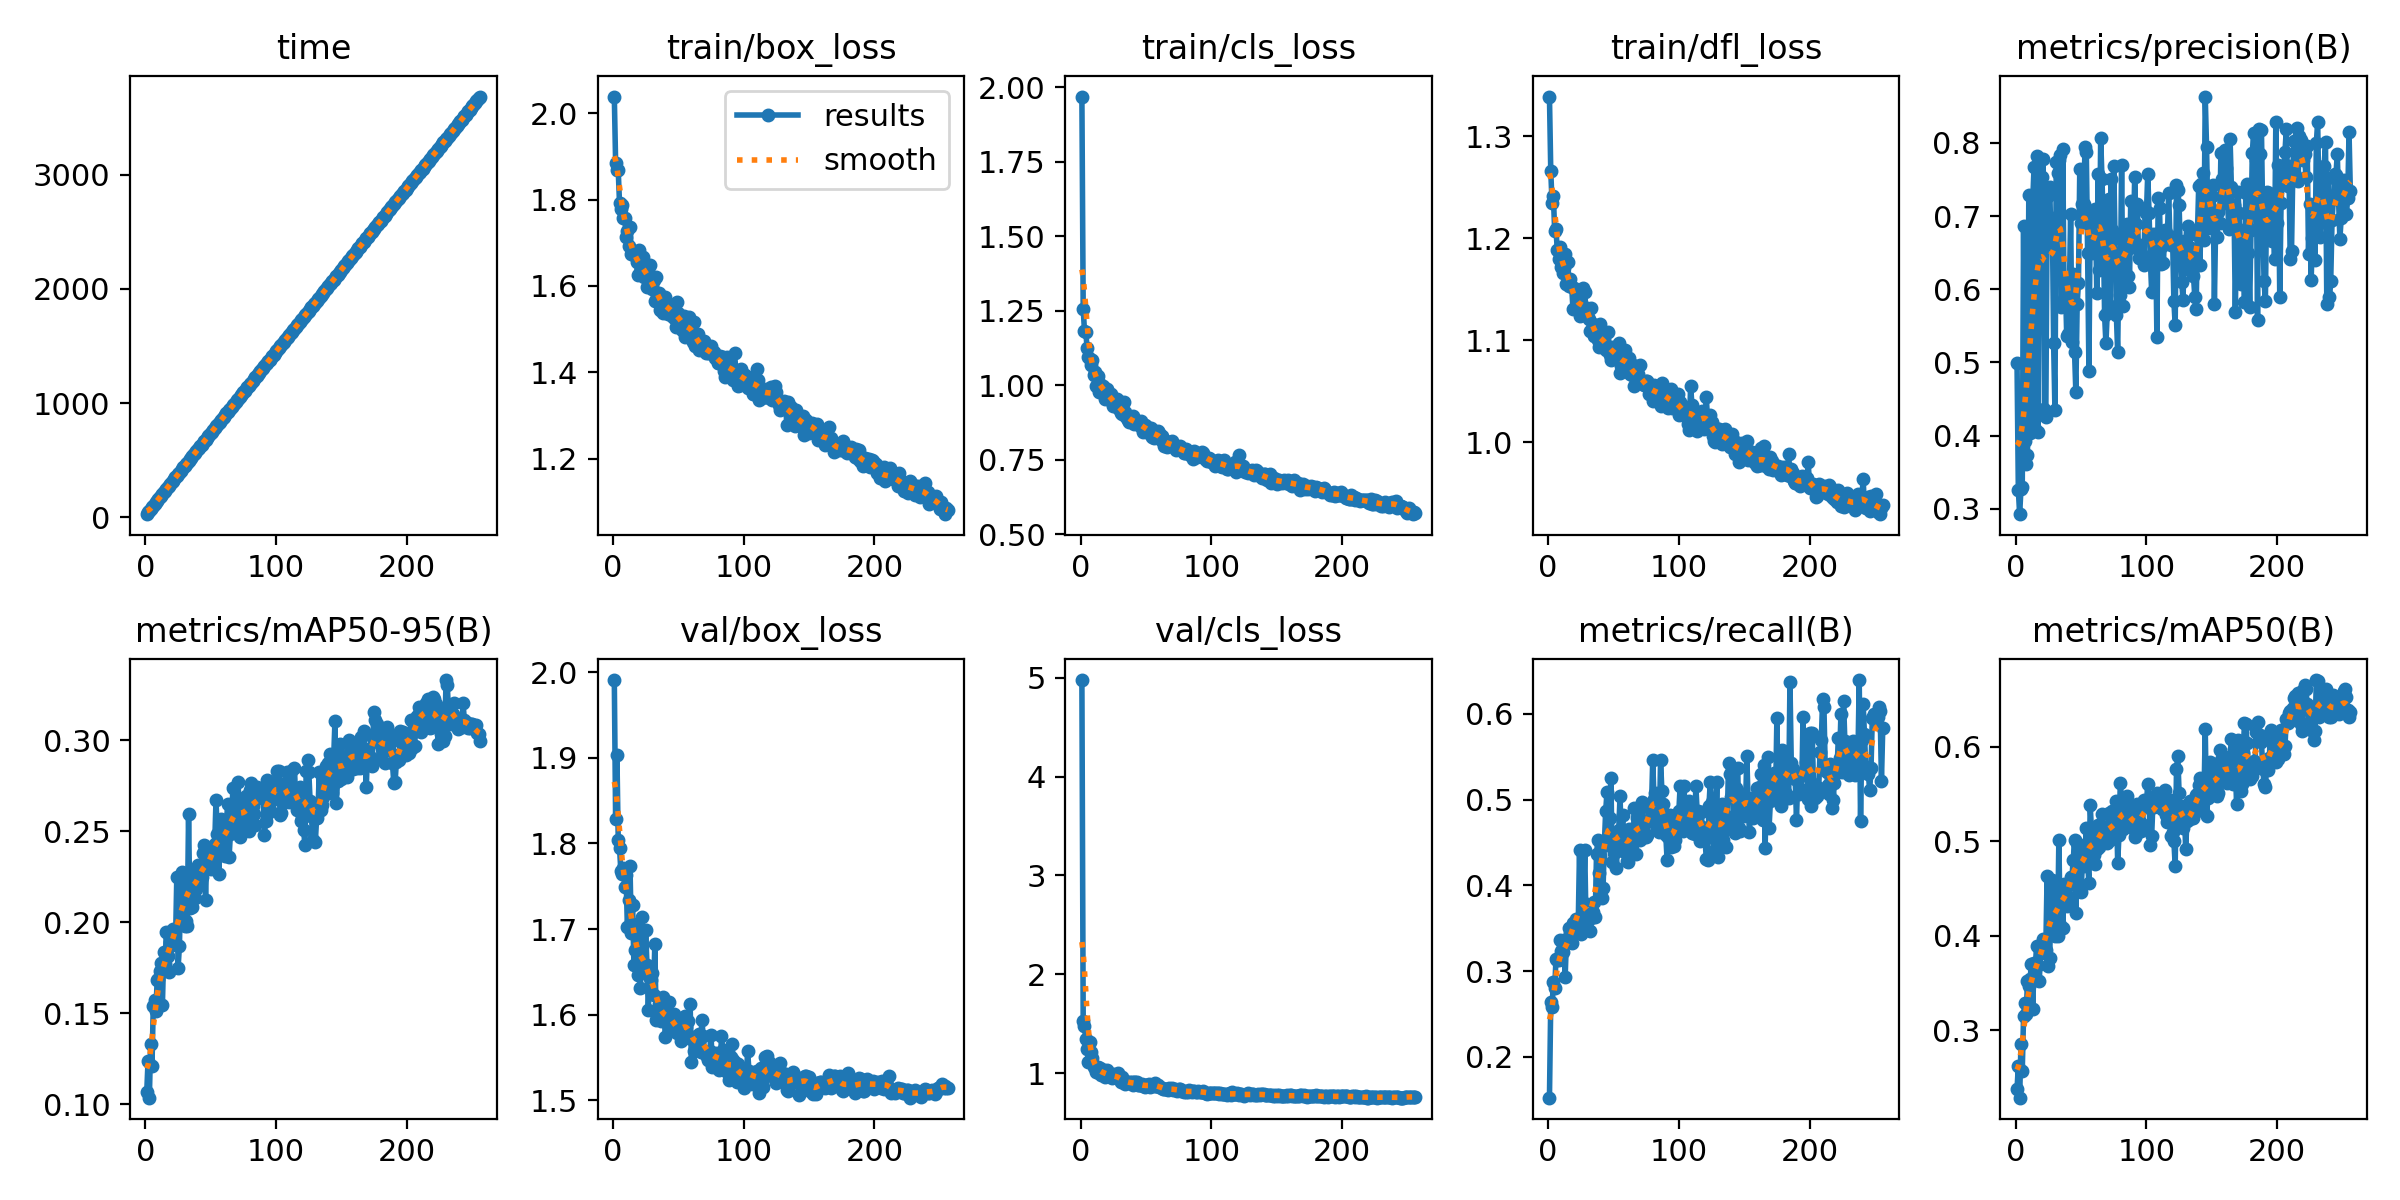
\includegraphics[width=0.9\textwidth]{15.png}
        \caption{Model progression over training epochs.}
        \label{fig:f8}
    \end{minipage}
\end{figure}




\begin{itemize}
    \item \textbf{Class Distribution}:
    \begin{itemize}
        \item The model has detected \textbf{107,004 vehicles}, which account for \textbf{62.5\%} of the total instances. This highlights the model's proficiency in identifying vehicles, which is expected given the prominence of vehicles in traffic scenes.
        \item \textbf{63,541 pedestrians} were detected, making up \textbf{37.1\%} of the total instances. This demonstrates that the model can effectively differentiate between pedestrians and vehicles.
        \item \textbf{781 emergency vehicles} were detected, representing only \textbf{0.5\%} of the total instances. While this is a small portion of the overall traffic, the low proportion reflects the inherent rarity of emergency vehicles in typical traffic datasets(see Fig \ref{fig:f6}).
    \end{itemize}

    \item \textbf{Bounding Box Analysis}:
    \begin{itemize}
        \item The model is highly accurate at identifying vehicles and pedestrians, as shown by the large number of bounding boxes correctly drawn for these categories.
        \item Emergency vehicle detection, while limited in quantity, is crucial. The lower number of emergency vehicles is expected given their scarcity, but improvements can still be made in this area to ensure all emergency vehicles are accurately detected in real-time.
    \end{itemize}

    \item \textbf{Model Accuracy}:
    \begin{itemize}
        \item With an accuracy of \textbf{79\%}, (mAP50) the model shows strong potential for practical deployment in real-world traffic management systems. However, there is still room for improvement, especially in fine-tuning the model's sensitivity to emergency vehicles, which are a critical class for priority-based traffic systems.
    \end{itemize}

    \item \textbf{Class Imbalance}:
    \begin{itemize}
        \item The data reflects an inherent imbalance in the dataset, with vehicles being the dominant class, followed by pedestrians. Emergency vehicles, being a rare class, may require special treatment in the training process (e.g., oversampling, data augmentation, or class weighting) to improve detection rates.
    \end{itemize}

    \item \textbf{Conclusion}:
    \begin{itemize}
        \item The current detection rates for vehicles and pedestrians are promising, while emergency vehicle detection remains a priority for further improvement. By focusing on fine-tuning the model and potentially introducing more emergency vehicle data into the training set, the system's accuracy and reliability can be further increased, particularly in scenarios where emergency vehicle prioritization is critical.
    \end{itemize}
\end{itemize}




Finally, after the implementation:

1. \textbf{Reduction in Vehicle Wait Time}:  
   The system will reduce average vehicle wait times by \textbf{33\%}, optimizing traffic flow through dynamic signal control in Bangladesh. This is especially important in Dhaka, where average speeds can drop to as low as 4.8 km/h during peak hours.

2. \textbf{Faster Emergency Vehicle Response}:  
   We hope after implementing the Emergency vehicle response times will reduced significantly. Because from research it seems up to \textbf{56\%} emergency vehicles are delayed due to traffic problems. So, real-time detection and prioritization of ambulances and fire trucks help people a lot. This improvement is crucial in Dhaka, where traffic congestion delays emergency services, creating life-threatening situations.

3. \textbf{Reduced Human Intervention}:  
   The system reduced the need for manual human effect, allowing for automated management based on real-time data footage. This minimized human error, ensuring smoother traffic flow, a major advantage given Dhaka’s dependency on traffic police.

4. \textbf{Prevention of Lane Starvation}:  
   By implementing starvation management techniques, the system prevented lanes from being blocked or underutilized for long periods, a frequent and hectic issue in Dhaka’s traffic congestion.

5. \textbf{Scalability and Reliability}:  
   The system’s use of hardware like Arduino, USB NodeMCU, and Raspberry Pi enabled reliable performance across multiple intersections without significant degradation, supporting its scalability for larger urban areas like Dhaka.

6. \textbf{Adaptability to Dynamic Traffic}:  
   The system adapted well to Dhaka’s unpredictable traffic patterns, such as sudden surges in traffic caused by events or road closures, ensuring real-time adjustments to minimize congestion and helping people a lot.

7. \textbf{Improved Public Safety and Efficiency}:  
   The prioritization of emergency vehicles (Ambulance, fire truck, etc) and the reduction in congestion significantly enhanced public safety and daily commuting efficiency, contributing to fewer delays and a smoother flow of traffic, which is critical in a densely populated city like Dhaka and other cities.

\section[]{Conclusion and Future Work}
In regard to traffic conditions of urban areas, the case study of methodology for automatic traffic control leverages machine learning and a diversity of identified algorithms to gain a more proficient, responsive, and intelligent automatic process for urban
traffic management systems on the road. This approach identifies the increasing challenges and difficulties of urban traffic congestion and aims to improve safety and ability at city intersections for the travelers and also ensure to reduction of the suffering because of traffic. In solving matters of traffic congestion the system’s adaptive abilities and its real-time data integration ensure that traffic is managed dynamically, and automatically, focusing on optimizing flow and increasing public safety on the road at a time. Future work will involve enhancing the system’s abilities to include more advanced fateful analytics exploring its integration with smart city initiatives and helping to find a solution after a high time.

\begin{thebibliography}{99}

\bibitem{clar:a1}
Kallol Mustafa, "Why exactly is Dhaka the slowest city in the world?" The Daily Star, Oct. 8, 2023. [Online]. Available: https://www.thedailystar.net/opinion/views/news/why-exactly-dhaka-the-slowest-city-the-world-3436751

\bibitem{clar:a2}
T. J. Karim, "Traffic Gridlock: Time Wasted in Dhaka," Dhaka Tribune, Dec. 5, 2022.

\bibitem{clar:a3}
Y. J. Yao, R. W. Yang, and L. Liu,(2020) "Design of Intelligent Traffic Management System Based on Video Detection Technology," IEEE Access, vol. 8, pp. 67278-67289.

\bibitem{clar:a4}
K. R. K. Singh, P. S. K. Prasad, and M. S. P. K. Roy, "Real-time Traffic Monitoring and Analysis Using YOLOv3 Model," Journal of Intelligent Transportation Systems, vol. 25, no. 5, pp. 509-520, 2021.

\bibitem{clar:a5}
Rahman, M. M., & Mohiuddin, M. (2020). "Traffic Management in Dhaka City: A Critical Review." Journal of Urban Planning and Development, 146(1), 04019029.

\bibitem{clar:a6}
Zhang, D., Wang, Y., & Liu, X. (2020). "Intelligent Traffic Light Control Using Deep Reinforcement Learning with Object Detection." IEEE Transactions on Intelligent Transportation Systems, 20(3), 1-10.

\bibitem{clar:a7}
J. D. J. Wu, M. R. Bell, and M. T. Williams, (2014). "The Effect of Traffic Congestion on Emergency Vehicle Response Times," Journal of Transportation Engineering, vol. 140, no. 8. [Online]. Available: https://ascelibrary.org/doi/abs/10.1061/(ASCE)TE.1943-5436.0000687

\bibitem{clar:a8}
Farooq, M., Habib, M. A., & Iqbal, M. (2020). "Priority-based Traffic Management System for Emergency Vehicles in Urban Areas." International Journal of Computer Applications, 175(20), 45-50.

\bibitem{clar:a9}
Ahmed, K., & Rahman, M. S. (2019). "Urban Traffic Congestion in Dhaka City: An Empirical Study." International Journal of Traffic and Transportation Engineering, 8(2), 19-30. 

\bibitem{clar:a10}
 Deccan Herald, Mar. 12, 2023. "AI-powered signals in Bengaluru reduce travel time by 33\%". [Online]. Available: https://shorturl.at/EEUsQ

\bibitem{clar:a11}
MM Hossain & A Kroeger. (2017). "87 Transport, delay to care and patient experience in pre-clinical emergency systems in dhaka city, bangladesh: a mixed methods study". [Online]. Available: https://shorturl.at/CpxTO

\bibitem{clar:a12}
N. Sharma, A. Garg, and P. Jain, (2021) "Smart traffic light control system using Raspberry Pi and IoT," International Journal of Computer Science and Network Security, vol. 21, no. 3, pp. 158-164.

\bibitem{clar:a13}
M. S. Islam, S. A. Chowdhury, and M. A. Hossain, (2020) "Design and implementation of an intelligent traffic control system using Arduino and machine learning," International Journal of Intelligent Systems and Applications, vol. 12, no. 4, pp. 42-50.

\bibitem{clar:a14}
J. Redmon, S. Divvala, R. Girshick, and A. Farhadi,(2016). "You Only Look Once: Unified, real-time object detection," Proceedings of the IEEE Conference on Computer Vision and Pattern Recognition (CVPR), pp. 779-788.

\bibitem{clar:a15}
C. Huang, Q. Liu, and D. Zhang,(2019). "YOLO-based traffic signal control system using deep reinforcement learning," Transportation Research Part C: Emerging Technologies, vol. 105, pp. 159-174.

\bibitem{clar:a16}
A. A. Gupta and S. R. Singh, (2020). "Impact of traffic congestion on emergency services in urban areas," International Journal of Transportation Science and Technology, vol. 10, no. 2, pp. 123-135.

\end{thebibliography}


% \label{lastpage}
\end{document}